\chapter{Matrix Element Method}
\label{sec:mem}
In the search for~\ttHbb, the irreducible~\ttbb~background presents an experimental challenge, as no single observable distinguishes between the signal and background process. Therefore, the information in multiple observables needs to be combined using multivariate analysis techniques (MVA), where the joint distribution of several observables is used to construct a discriminator between the signal and background process hypotheses.

In the following chapter, we will describe the implementation of a multivariate technique that is based on the direct computation of theory-motivated likelihoods for the observations using the underlying matrix element for the hard scattering process. The matrix element method (MEM) thus allows to connect the observable quantities at the detector level, such as jet or lepton momenta, to the dynamics of the scattering process. We show that the MEM provides a suitable framework for interpreting data from multi-parton final states and it can be used to construct a discriminator between irreducible processes that is theoretically motivated and practical for analysis.

We will motivate the MEM approach from a statistical point of view and describe the theoretical background of the MEM likelihood. Furthermore, we discuss in detail the improvements made to the MEM as applies to the~\ttHbb~analysis in Run II, where we have extended the method to incorporate effects from mis-reconstructed jets and additional QCD radiation. This considerably extended the phase space which can be analysed using the MEM technique. Finally, we study the expected performance of the MEM in simulation.

\section{Hypothesis testing}
\label{sec:test_statistic}
We can formulate the problem of deciding if an event as arose from a signal or background process as a binary classification. We distinguish between the background hypothesis~($H_0$) and signal hypothesis ($H_1$) on an event-by-event basis based on the observables~$\vec{y}$. We classify an event as signal by rejecting the hypothesis~$H_0$ in favour of~$H_1$. In the framework of statistical hypothesis testing, we define a function~$\lambda(\vec{y})$, the test statistic, for which the sampling distributions under the hypotheses can be estimated using MC simulation. Based on the observed value of $\lambda(\vec{y})$ for an event, we decide if it should be interpreted as signal or background. In practice, the we use the continuous value of the test statistic in a template fit. The choice of the test statistic determines the size of the test, i.e. the probability of falsely rejecting~$H_0$ if it is true, and the power of the test, which is the probability of rejecting the null hypothesis in case it is false.

In case we are dealing with two simple hypotheses that do not depend on additional parameters, the Neyman-Pearson lemma~\cite{neyman1992problem} states that the likelihood ratio

\begin{equation}
\lambda(\vec{y}) = \frac{L(\vec{y}|\mathrm{H}_1)}{L(\vec{y}|\mathrm{H}_0)}
\end{equation}
is the most powerful test statistic. Therefore, the task of computing the likelihood~$L(\vec{y}|\mathrm{H}_i)$ of an observation characterized by~$\vec{y}$ under a given hypothesis is central to binary classification. Naively, this could be achieved using MC simulation to estimate the multidimensional probability density~$f(\vec{y}|\mathrm{H}_i)$ and using it as the likelihood, however, this quickly becomes intractable as the dimensionality of~$\vec{y}$ increases. Fortunately, the underlying theory of particle physics provides a way to compute probability densities in the form of differential cross section for processes involving scattering and interactions. In the next section, we will discuss how we can construct a useful likelihood function~$L(\vec{y}|\mathrm{H})$ using the theoretical framework provided by QFT.

\section{Description of MEM}

The use of MVA techniques has a long history in HEP data analysis, starting with multivariate discriminators in the analysis of bubble chamber data~\cite{VanDoninck:1984wd} and investigations of artificial neural networks (ANN) for tracking~\cite{Denby:1987rk}. Traditional methods are based on likelihood ratios constructed from 1-dimensional distributions estimated form simulation, which do not properly account for the correlations between variables, or machine learning (ML) techniques such as BDTs or ANNs. The advantage of the ML based methods is that they can faithfully approximate complex functions, however, they suffer from several important drawbacks:

\begin{itemize}
\item in HEP, such ML methods are optimized completely on simulation, making the prediction susceptible to over-fitting in case the model does not represent data accurately
\item they require extensive MC simulation to be optimized effectively, such that $\mathcal{O}(10^8)$ MC events are routinely simulated with full detector simulation to have sufficient statistics in high jet multiplicity categories.
\item the predictions are often opaque, combining dozens of variables in complex ways, such that it is not generally possible to analyze why an event was classified as signal or background.
\end{itemize}
Therefore, we seek an alternative that would be less susceptible to the aforementioned issues.

The MEM belongs to a class of MVA methods in which we directly compute the per-event probability density that depends on model parameters~$\vec{\theta}$ from first principles via

\begin{equation}
P_{\vec{\theta}}(\vec{y}) = \frac{1}{\sigma}
\frac{\mathrm{d}\sigma_{\vec{\theta}}(\vec{y})}{\mathrm{d}\vec{y}}
\end{equation}
and use it in hypothesis testing as component of the test statistic. Through the differential cross section, the MEM explicitly depends on~$\vec{y} = (\tilde{p}_{i \in \mathrm{jets}}, \tilde{p}_{i \in \mathrm{leptons}}, \dots)$, the vector containing the detector-level 4-momenta of the reconstructed particles, in particular, jets and leptons. The differential cross-section~(\cref{eq:diff_cross_section}) depends on the squared matrix element~$|\mathcal{M}^2|$ that we use to take into account the dynamics of the relevant underlying processes. The kinematics of the~$2 \rightarrow n$ scattering process are encoded in the~$n$-body phase space element~(\cref{eq:n_body_phase_space}), where the delta function enforces the conservation of momentum between the initial and final state particles.

\begin{equation}
\label{eq:diff_cross_section}
\mathrm{d}\sigma_{\vec{\theta}} = \frac{(2\pi)^4 |\mathcal{M}_{\vec{\theta}}|^2}{4 \sqrt{(q_1 \cdot q_2)^2 - m_1 m_2}} \times
\mathrm{d}\Phi_n(q_1 + q_2; p_1, \dots, p_{n})
\end{equation}

\begin{equation}
\label{eq:n_body_phase_space}
\mathrm{d}\Phi_n = \delta^4 (q_1 + q_2 - \sum_{i=1}^n p_i) \prod_{i=1}^n \frac{\mathrm{d}^3 p_i}{(2\pi)^3 2 E_i}
\end{equation}

We have to consider several additional effects to be able to compute~$P_{\vec{\theta}}(\vec{y})$:
\begin{itemize}
\item We cannot directly observe the momenta of the initial state particles~$q_1$ and~$q_2$ in a proton-proton collision.
\item We do not measure the momenta of the neutrinos or jets that do not pass a transverse momentum threshold and the detector has a finite energy resolution.
\item We do not know which of the observed jets are matched to which partons.
\item The non-zero final transverse momentum caused by large-angle initial state radiation, spoiling the momentum balance in~\cref{eq:n_body_phase_space}.
\end{itemize}

To address the first issue, we need to use parton density functions~$g(x_{1,2})$ to weight the differential cross-section, integrating over the momentum fractions~$x_{1,2} = E_{q_{1,2}}/E_{\mathrm{beam}}$.
In order to take into account detector effects, we integrate over unmeasured or poorly measured quantities using a transfer function~$W(\vec{y}, \vec{p})$.
The transfer function relates final state parton-level quantities~$\vec{p}$ to measurable quantities on the detector level~$\vec{y}$ and encodes our knowledge about detector resolution or reconstruction efficiencies.

The question of jet-to-parton matching is addressed by summing over the~$N_a$ possible combinations of jet-to-parton matching, which depends on assumptions about the process and the number of observed final state particles and is encoded in the exact factorized form of the transfer function~$W(\vec{y}, \vec{p})$.

Finally, the modelling of the non-zero transverse recoil~$\vec{\rho}_T = -\sum_{i=1}^n \vec{p}_{i,T}$ is treated empirically using a transfer function~$\mathcal{R}(\tilde{\vec{\rho}}_T, \vec{\rho}_T)$ determined on simulation that relates the parton-level transverse momentum of the system~$\vec{\rho}_T$ to the observed recoil~$\tilde{\vec{\rho}}_T$. 

The evaluation of~$|\mathcal{M}_{\vec{\theta}}(\vec{p})|^2$ requires full knowledge of the initial and final state momenta~$\vec{p}$, as well as the parameters of the model, summarized in~$\vec{\theta}$. In particular, the parameters of the model consist of the hypothesis~$\mathcal{H} \in \{\ttH, \ttbb\}$ about the underlying process and the assumptions about which of the partons formed reconstructed jets~$\mathcal{C}$, such that~$\vec{\theta} = (\dots, \mathcal{H}, \mathcal{C})$. In the case of~\ttH~with the top quark pair decaying semileptonically~$\ttH \rightarrow (\ell^- \bar{\mathrm{\nu}}_\ell \mathrm{b})\ (\mathrm{q} \mathrm{q}' \bar{\mathrm{b}})\ (\mathrm{b} \bar{\mathrm{b}})$, we may consider the fully reconstructed category where all 6 of the final state partons are reconstructed as jets, denoted as~$2_W 2_H 2_t$, the case where one of the quarks from the hadronic decay~$\mathrm{W} \rightarrow \mathrm{q} \mathrm{q}'$ is out of acceptance, denoted as~$1_W 2_H 2_t$ and so forth, such that~$\mathcal{C}_{\mathrm{SL}} \in \{ 2_W 2_H 2_t, 1_W 2_H 2_t, \dots \}$. The number of unknown quantities to be integrated over depends on the reconstruction category~$\mathcal{C}$, as described in detail in the next section. 
Thus, the per-event probability density takes the form

\begin{align}
\label{eq:mem_definition}
P(\vec{y}, \vec{\theta}) &= \sum_{k=1}^{N_a} \int \frac{\mathrm{d}x_1 \mathrm{d}x_2}{2 x_1 x_2 s} \int \prod_{i=1}^{n} \frac{\mathrm{d}^3 p_i}{(2\pi)^3 2 E_i} \\
&\times \delta^4 (q_1 + q_2 - \sum_{i=1}^n p_i)\\
&\times g(x_1) g(x_2) \\ 
&\times \mathcal{R}(\tilde{\vec{\rho}}_T, \vec{\rho}_T) \\ 
&\times |\mathcal{M}_{\vec{\theta}}(q_1, q_2, p_1, \dots, p_n)|^2 \\
&\times W(\vec{y}, \vec{p}).
\end{align}

After having been first proposed for reconstructing events with missing momentum~\cite{Kondo:1988yd}, the MEM has been used in Tevatron for Higgs boson searches~\cite{Aaltonen:2009dh,Aaltonen:2011rt} and a precise measurement of the top quark mass~\cite{D0topmass2004}. After first phenomenological studies showed that MEM could be used effectively for~\ttH~in a multi-parton final state~\cite{Artoisenet:2013vfa}, it has been used in searches for~\ttHbb~by the CMS and ATLAS experiments in Run I of the LHC\cite{Aad:2015gra,Khachatryan:2015ila}. The MEM approach is closely related to the matrix element likelihood approach (MELA)~\cite{Gao:2010qx} that has been extensively used in~$\mathrm{H} \rightarrow \mathrm{ZZ} \rightarrow 4\mathrm{l}$ searches and~$J^P$ measurements, however, in MELA, unreconstructed particles and transfer functions are not considered and the matrix elements generally have simple analytical forms.
In the following sections, we discuss in detail the implementation and improvements that were made to the MEM in the search for~\ttHbb~during Run II.

\section{Implementation}
\label{sec:mem_implementation}
In the case of semileptonic or dileptonic~\ttH~final state, the observables~$\vec{y}$ consist of the energies (or equivalently transverse momenta) and the directions of the jets, the momenta of the charged leptons and the measured recoil of the system~$\tilde{\vec{\rho}}_T$. As~\cref{eq:mem_definition}~needs to be integrated numerically, we first need to define the phase space volume element explicitly in terms of variables that are convenient and suitable for integration, namely energies, solid angles and combinations of invariant masses. The Jacobian transformation can be done analytically for all particles and are of the form shown in~\cref{eq:phase_space_jacobian} for the~\Hbb~decay, the unassociated~$\mathrm{b}\bar{\mathrm{b}}$ from~\ttbb~ and the top decay with~$qq'$ corresponding to the quarks or leptons from the~$\mathrm{W}$ boson decay:

\begin{align}
\label{eq:phase_space_jacobian}
\Hbb:\ \prod_{i=1}^{2} \frac{\mathrm{d}^3 p_i}{(2\pi)^3 2 E_i} =& \biggr(\frac{1}{16 \pi^3}\biggl)^2 \times \frac{p_b p_{\bar{b}}}{8 |E_b - \vec{p}_b \cdot \frac{\vec{e}_{\bar{b}}}{\beta_{\bar{b}}}|} \times \\
&\times\mathrm{d}E_{b}~\mathrm{d}m^2_{b\bar{b}}~\mathrm{d}\Omega_{b}~\mathrm{d}\Omega_{\bar{b}} \\
\mathrm{b}\bar{\mathrm{b}}:\ \prod_{i=1}^{2} \frac{\mathrm{d}^3 p_i}{(2\pi)^3 2 E_i} =& \biggr(\frac{1}{16 \pi^3}\biggl)^2 \times \frac{p_b p_{\bar{b}}}{4}~\mathrm{d}E_{b}~\mathrm{d}E_{\bar{b}}~\mathrm{d}\Omega_{b}~\mathrm{d}\Omega_{\bar{b}} \\
\mathrm{t} \rightarrow \mathrm{b}\mathrm{q}\mathrm{q}':\ \prod_{i=1}^{3} \frac{\mathrm{d}^3 p_i}{(2\pi)^3 2 E_i} =& \biggr(\frac{1}{16 \pi^3}\biggl)^3 \times \frac{p_q p_{q'} E_{q'}}{16 m_{qq'}^2 |(E_q + E_{q'}) - (\vec{p}_q + \vec{p}_{q'})\cdot \frac{\vec{e}_b}{\beta_b}|}\times\\
&\times\mathrm{d}E_{q}~\mathrm{d}m^2_{qq'}~\mathrm{d}m^2_{qq'b}~\mathrm{d}\Omega_{q}~\mathrm{d}\Omega_{q'}~\mathrm{d}\Omega_b,
\end{align}
where we have expressed the Lorentz-invariant phase space in terms of particle energies, angles ($\mathrm{d}\Omega = \sin{\theta}~\mathrm{d}\theta~\mathrm{d}\phi$) and invariant masses~$m_{qq'} = (q+q')^2$,~$m_{qq'b} = (q + q' + b)^2$.
The scattering amplitude written as~$|\mathcal{M}(\vec{p})|^2$ depends only on particle momenta, hence it is implied to be summed over spin and colour states. Furthermore, we treat the production and decay of the top quarks, W and Higgs bosons in the narrow-width approximation (NWA), meaning we factorize the production and decay of these particles, as seen in~\cref{eq:scattering_nwa}.

\begin{align}
\label{eq:scattering_nwa}
|\mathcal{M}_{\ttH \rightarrow (qq'b) (qq'\bar{b}) (b\bar{b})}|^2 &= |\mathcal{M}_{gg \rightarrow~\ttH}(g_1, g_2, t, \bar{t}, h)|^2 \\
&\times \prod_{r = t,\bar{t}} \bigl[ \frac{\pi}{m_t \Gamma_t} \delta(t^2 - m_t^2) |\mathcal{M}_t(q,\bar{q},b)|^2 \bigr]_r \\
&\times \frac{\pi}{m_t \Gamma_t} \delta(h^2 - m_H^2) |\mathcal{M}_H(b,\bar{b})|^2
\end{align}

The decay amplitude of the top quark, assuming the NWA for the W-boson, is given in~\cref{eq:decay_top}

\begin{equation}
\label{eq:decay_top}
|\mathcal{M}_t(q,q',b)|^2 = \frac{32\pi m_t^4 g^4}{m_W \Gamma_W} {2 q\cdot t}{m_t^2} (1 - \frac{m_b^2}{m_t^2} - \frac{2 q \cdot t}{m_t^2}) \times \delta((q+q')^2 - m_W^2)
\end{equation}
and for the~$\mathrm{H} \rightarrow \mathrm{b}\bar{\mathrm{b}}$ in~\cref{eq:decay_higgs}:

\begin{equation}
\label{eq:decay_higgs}
|\mathcal{M}_H(b,\bar{b})|^2 = 2\sqrt{2} m_b^2 m_H^2 (1 - \frac{4m_b^2}{m_H^2}).
\end{equation}

\subsection{Transfer functions}
\label{sec:transfer_functions}

The transfer function~$W(\vec{y} | \vec{p})$ maps a point~$\vec{p} \in \Omega$ in the phase space of the hard scattering process to a point~$\vec{y} \in \mathcal{A}$ in the space of detector-level reconstructed variables and it is ensured to be normalized to unity using~\cref{eq:transfer_normalization},

\begin{equation}
\label{eq:transfer_normalization}
\int_{\mathcal{A}} \mathrm{d}\vec{y}~W(\vec{y} | \vec{p}) = 1,
\end{equation}
which means that in an observable fiducial region $\mathcal{A}^* \subset \mathcal{A}$, a phase space point has an efficiency~$\epsilon(\vec{p}) \leq 1$ to be reconstructed. We note that since the same transfer functions are applied for all hypotheses, the choice of transfer functions ultimately affects the model sensitivity, but not the correctness, that is, we are not introducing any bias into the analysis with our assumptions.

We can make further progress by factorizing the transfer function in terms of individual reconstructed objects, the jets and leptons:

\begin{equation}
W(\vec{y} | \vec{p}) = \prod_{i\in \mathrm{jets}} W(E_i, \vec{e}_i | E_{q_i}, \vec{e}_{q_i})
\prod_{i\in \ell^\pm} W(E_i, \vec{e}_i | E_{\ell_i}, \vec{e}_{\ell_i}) = \prod_{i \in \mathrm{jets}} W_{i,j} \prod_{i \in \ell^\pm} W_{i,\ell},
\end{equation}
where~$q_i$ ($\ell_i$) is shorthand for the quark (charged lepton) assumed to give rise to the~$i$-th measured jet (charged lepton). If we are dealing with indistinguishable objects such as jets, we have to sum over all possible ways of matching the detector-level and parton-level objects, such that

\begin{equation}
\label{eq:tf_combination_sum}
W_{i,j} \propto \sum_{q_i \in \mathrm{quarks}} W(E_i, \vec{e}_i | E_{q_i}, \vec{e}_{q_i}).
\end{equation}
In particular, we make no assumption on jet charge, therefore, to assign out of 4 reconstructed b-jets 2 to the quarks from~$\Hbb$, we have~$4!/2!2! = 6$ combinations. Without distinguishing between~$\mathrm{b}$ and~$\bar{\mathrm{b}}$, we have a further~$2!/1!1!$ ways of assigning the b~tagged jets to bottom quarks from the top or antitop quarks, such that assigning the fully reconstructed~\ttHbb~hypothesis with 4 b~quarks and 2 light quarks among 6 jets amounts to 12 combinations. We describe the approach taken to reducing the number of required combinations further in~\cref{sec:event_interpretation}.

Lepton energies and directions are measured with an order of magnitude higher resolution than jet energies, therefore we assume those to be perfectly measured so that their transfer functions are Dirac delta functions.
Furthermore, we assume that the jet energy and angular transfer functions can be factorized such that

\begin{equation}
W(E_i, \vec{e}_i | E_{q_i}, \vec{e}_{q_i}) = W(E_i | E_{q_i}) \times W(\vec{e}_i | \vec{e}_{q_i})
\end{equation}
and that jet directions are measured much more accurately than jet energies.
With these assumptions, the transfer function for observed particles reduces to a product of~$W(E_i | E_{q_i})$ over the jets.

We use a double Gaussian function, shown in~\cref{eq:double_gaussian},

\begin{equation}
\label{eq:double_gaussian}
W(p_{T,j} | p_{T,\mathrm{gen}}) = N \biggl[0.7\exp{\biggl(\frac{p_{T,\mathrm{gen}} - p_{T,j} - \alpha_1}{\alpha_2}\biggr)^2} + 0.3\exp{\biggl(\frac{p_{T,\mathrm{gen}} - p_{T,j} - \alpha_3}{\alpha_2+\alpha_4}\biggr)^2}\biggr],
\end{equation}
to model the parton-to-jet transfer function for both light jets and b~jets.

The parameters of these transfer functions are derived from MC simulation, assuming that they depend on quark energy, direction and flavour. We extract the transfer functions from a~\ttbar~MC sample by matching the generator-level partons geometrically to jets using~$\Delta R(q,j) < 0.3$ and performing fits of the~$W(p_{T,j}|p_{T,q})$ distributions. We fit the parameters~$\alpha_1 \dots \alpha_4$ of~\cref{eq:double_gaussian} in bins of~$p_{T,q}$,~$|\eta_{q}|$ and flavour~$\mathrm{f}\in{\mathrm{l}, \mathrm{b}}$, shown on~\cref{fig:transfer_perbin}. Additionally, in order to have a smooth dependence of the transfer functions on~\ptgen~, we fit polynominals to the per-bin parameters~$\alpha_n(\ptgen|\eta_{q},\mathrm{f})$, shown on~\cref{fig:transfer_acrossbin} for b~jets in the central detector region~$0 < |\eta| \le 1.0$. Thus, we are able to evaluate the probability density for a quark with~$\ptgen,\eta$ to hadronize into a jet continuously over the full range of~$\ptgen$.

\begin{figure}
\begin{centering}
\subfloat[Fit for b~jets.]{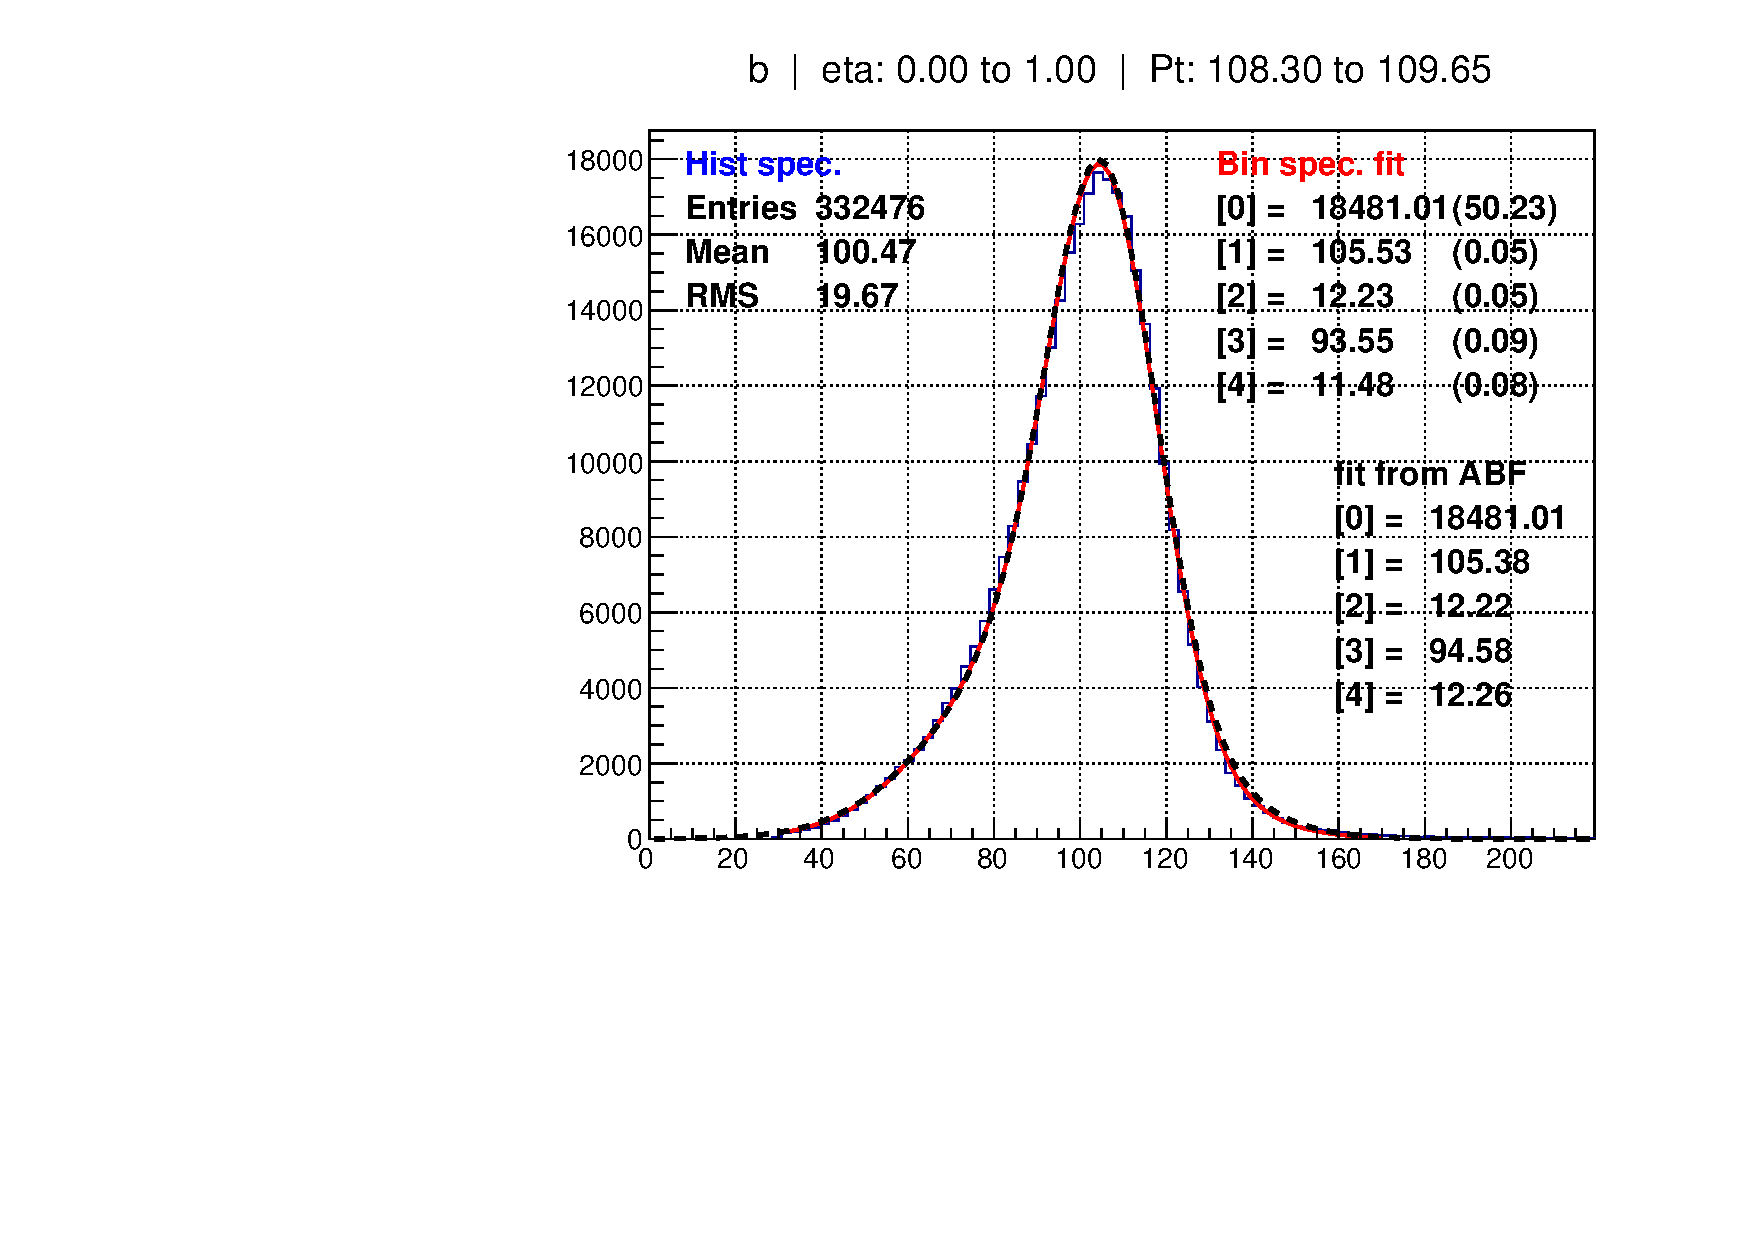
\includegraphics[width = 0.5\textwidth]{figures/transfer/b-0-32.pdf}}
\subfloat[Fit for light jets.]{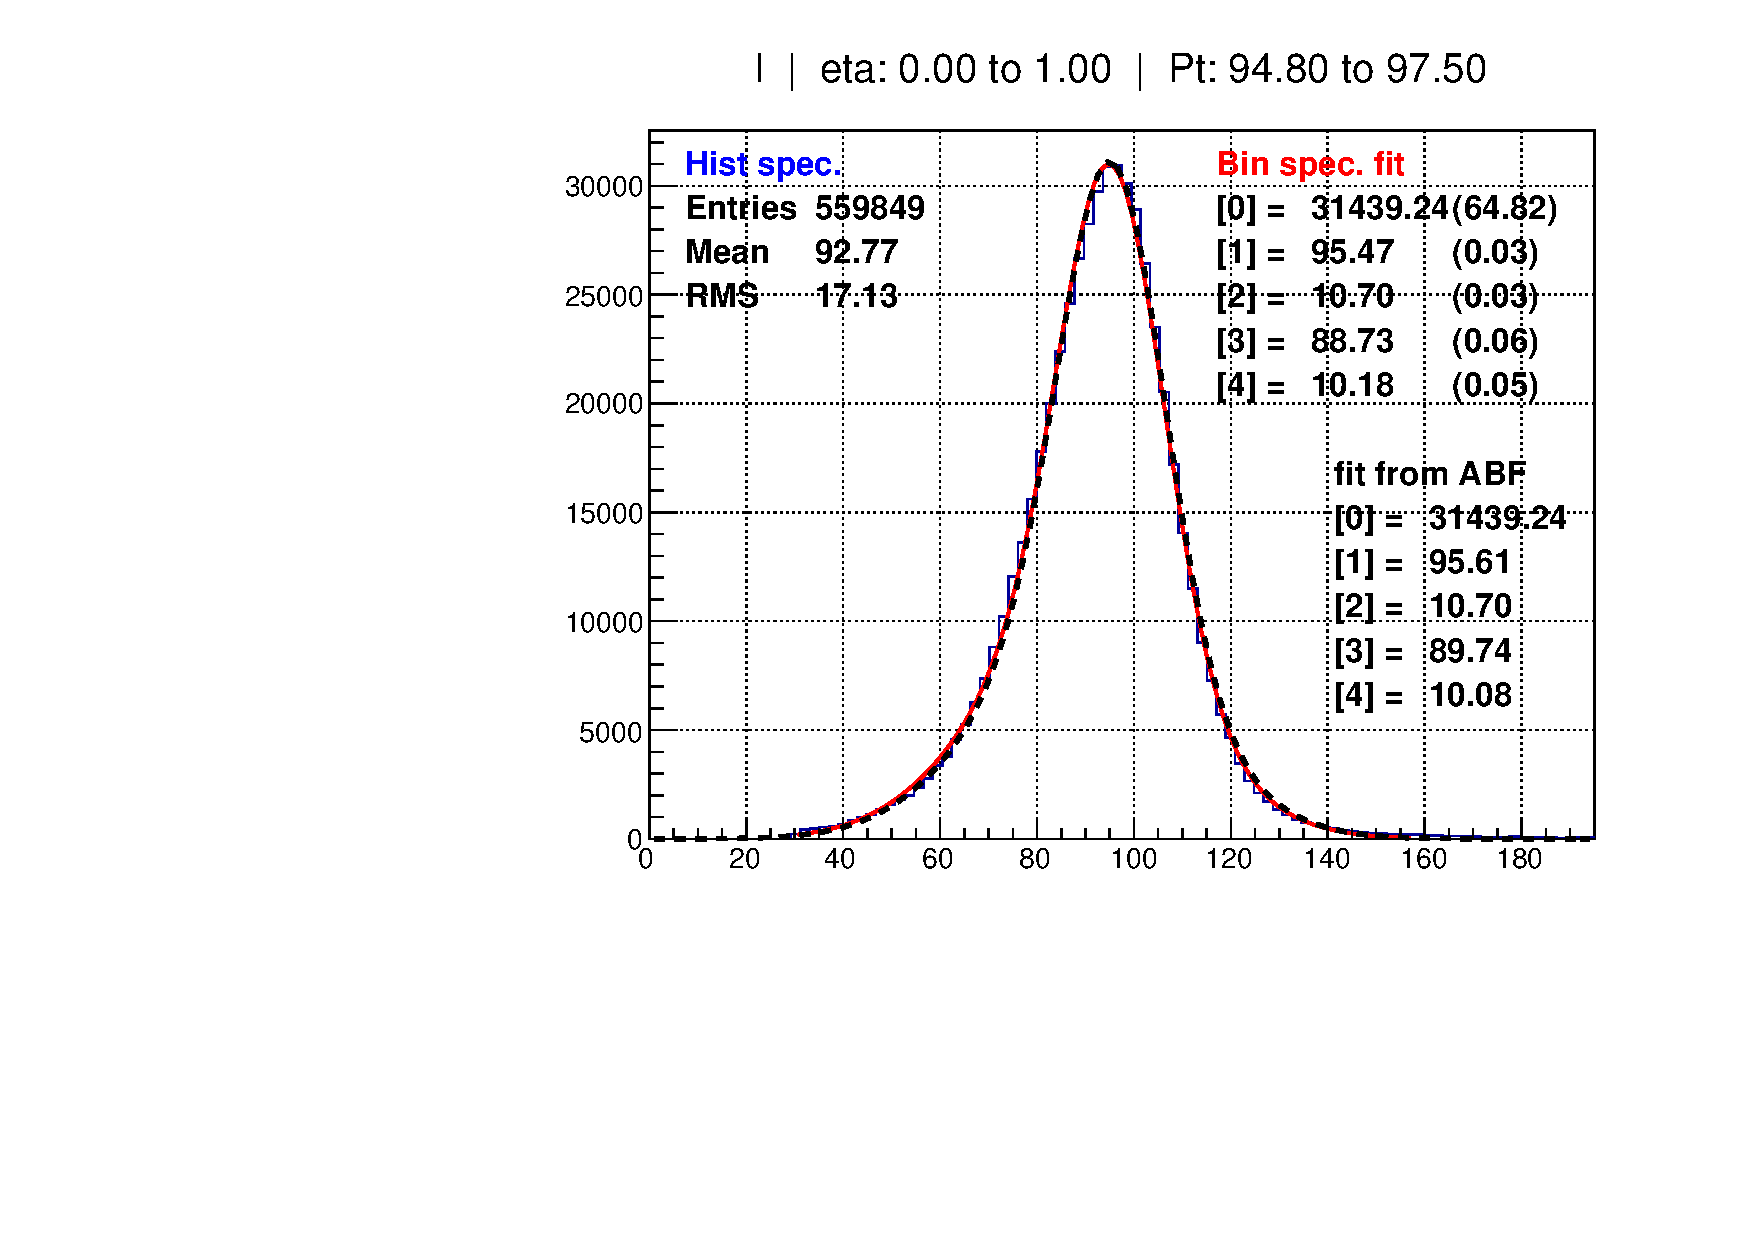
\includegraphics[width = 0.5\textwidth]{figures/transfer/l-0-32.pdf}} \\
\caption[The double-Gaussian transfer function fit in~\ttbar~simulation.]{The double Gaussian~(\cref{eq:double_gaussian})~fit (red) to the simulated transfer function (light blue) for b~jets~(\textbf{a}) and light jets~(\textbf{b}) in the central detector region~($0 < |\eta| \le 1$) in a~$\ptgen \simeq 100$ GeV region. In general, we see that the double Gaussian function is sufficiently flexible to describe the transfer functions for both light jets and b~jets. Furthermore, the interpolated double Gaussian using the fitted parameters~$\alpha_1 \dots p_4$ (black) reproduces the exact double Gaussian fit reasonably well. The plots are derived using~\ttbar+jets simulation.}
\label{fig:transfer_perbin}
\end{centering}
\end{figure}

\begin{figure}
\begin{centering}
\subfloat[Fit of~$p_1$.]{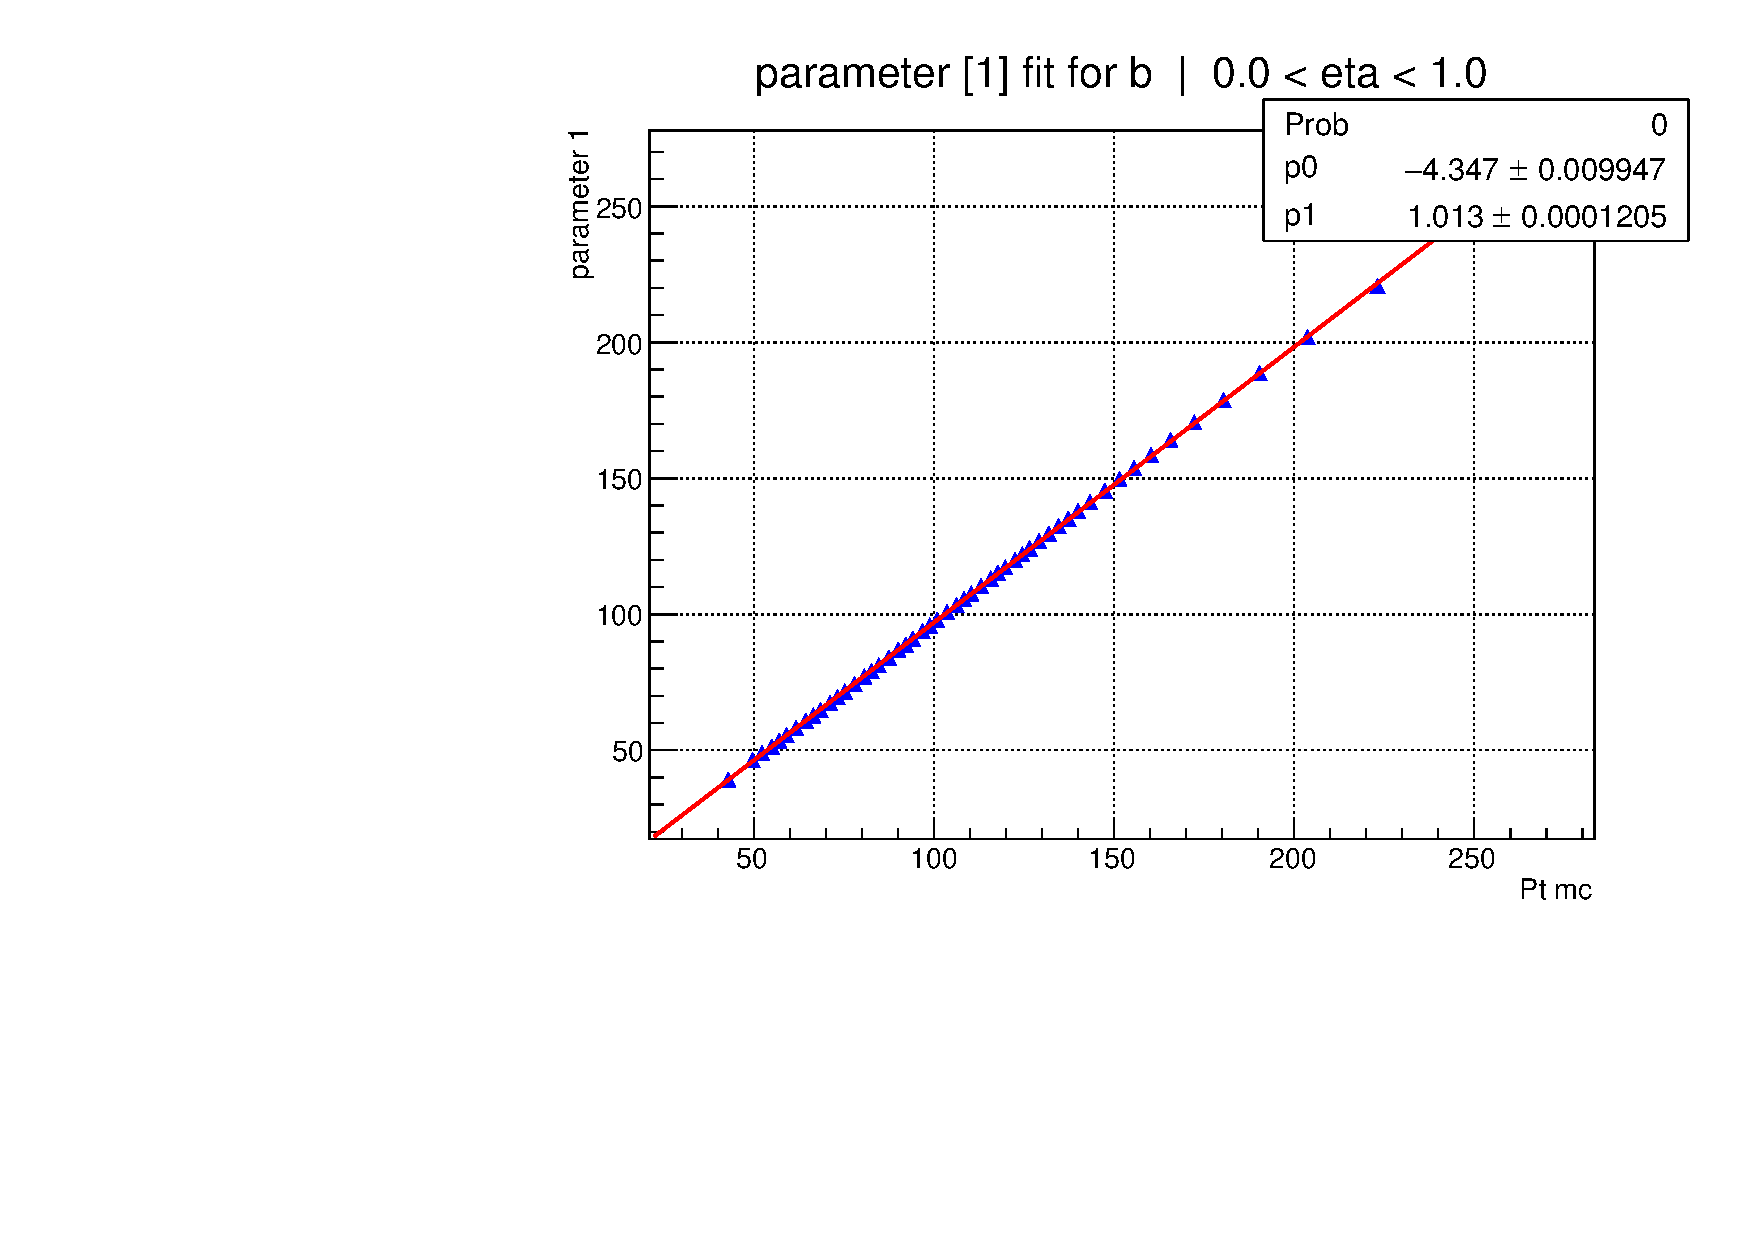
\includegraphics[width = 0.5\textwidth]{figures/transfer/par1-b-eta0.pdf}}
\subfloat[Fit of~$p_2$.]{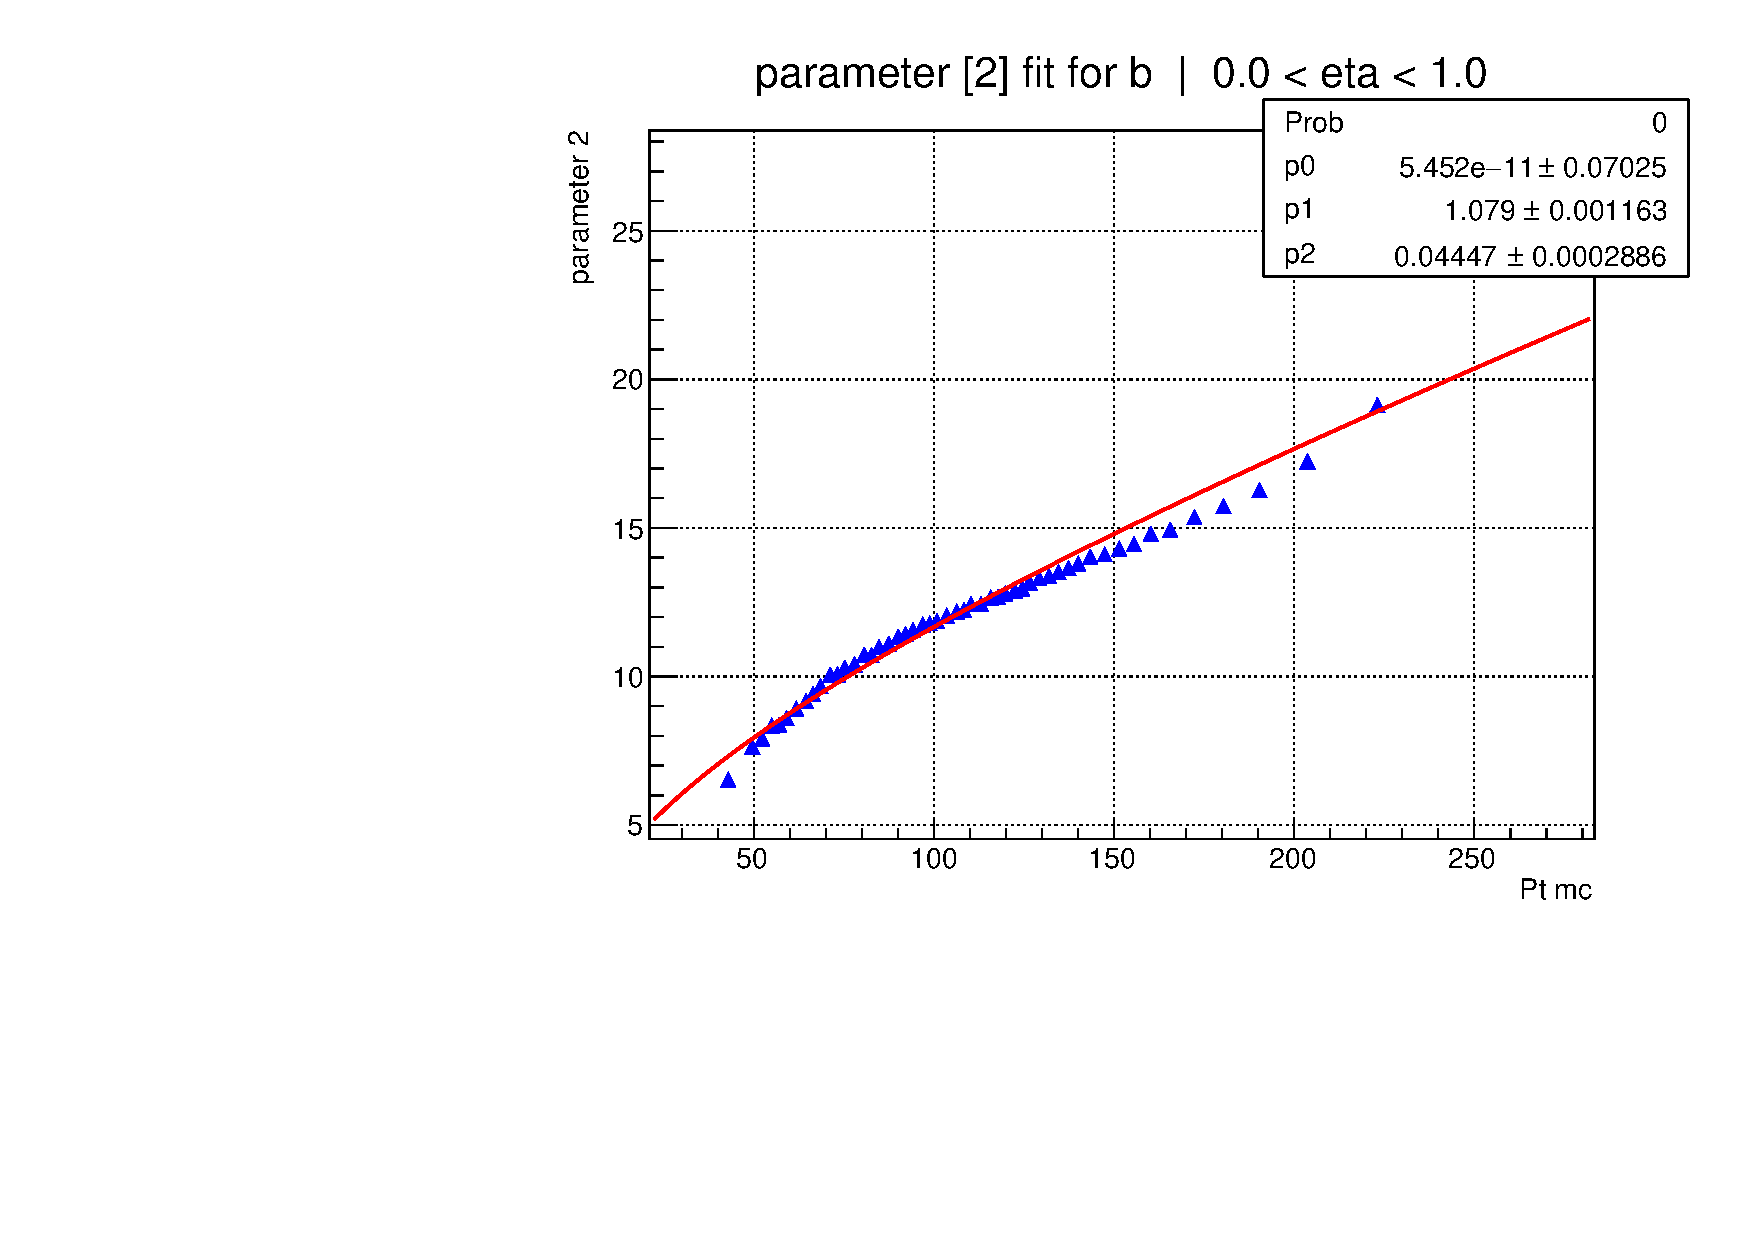
\includegraphics[width = 0.5\textwidth]{figures/transfer/par2-b-eta0.pdf}} \\
\subfloat[Fit of~$p_3$.]{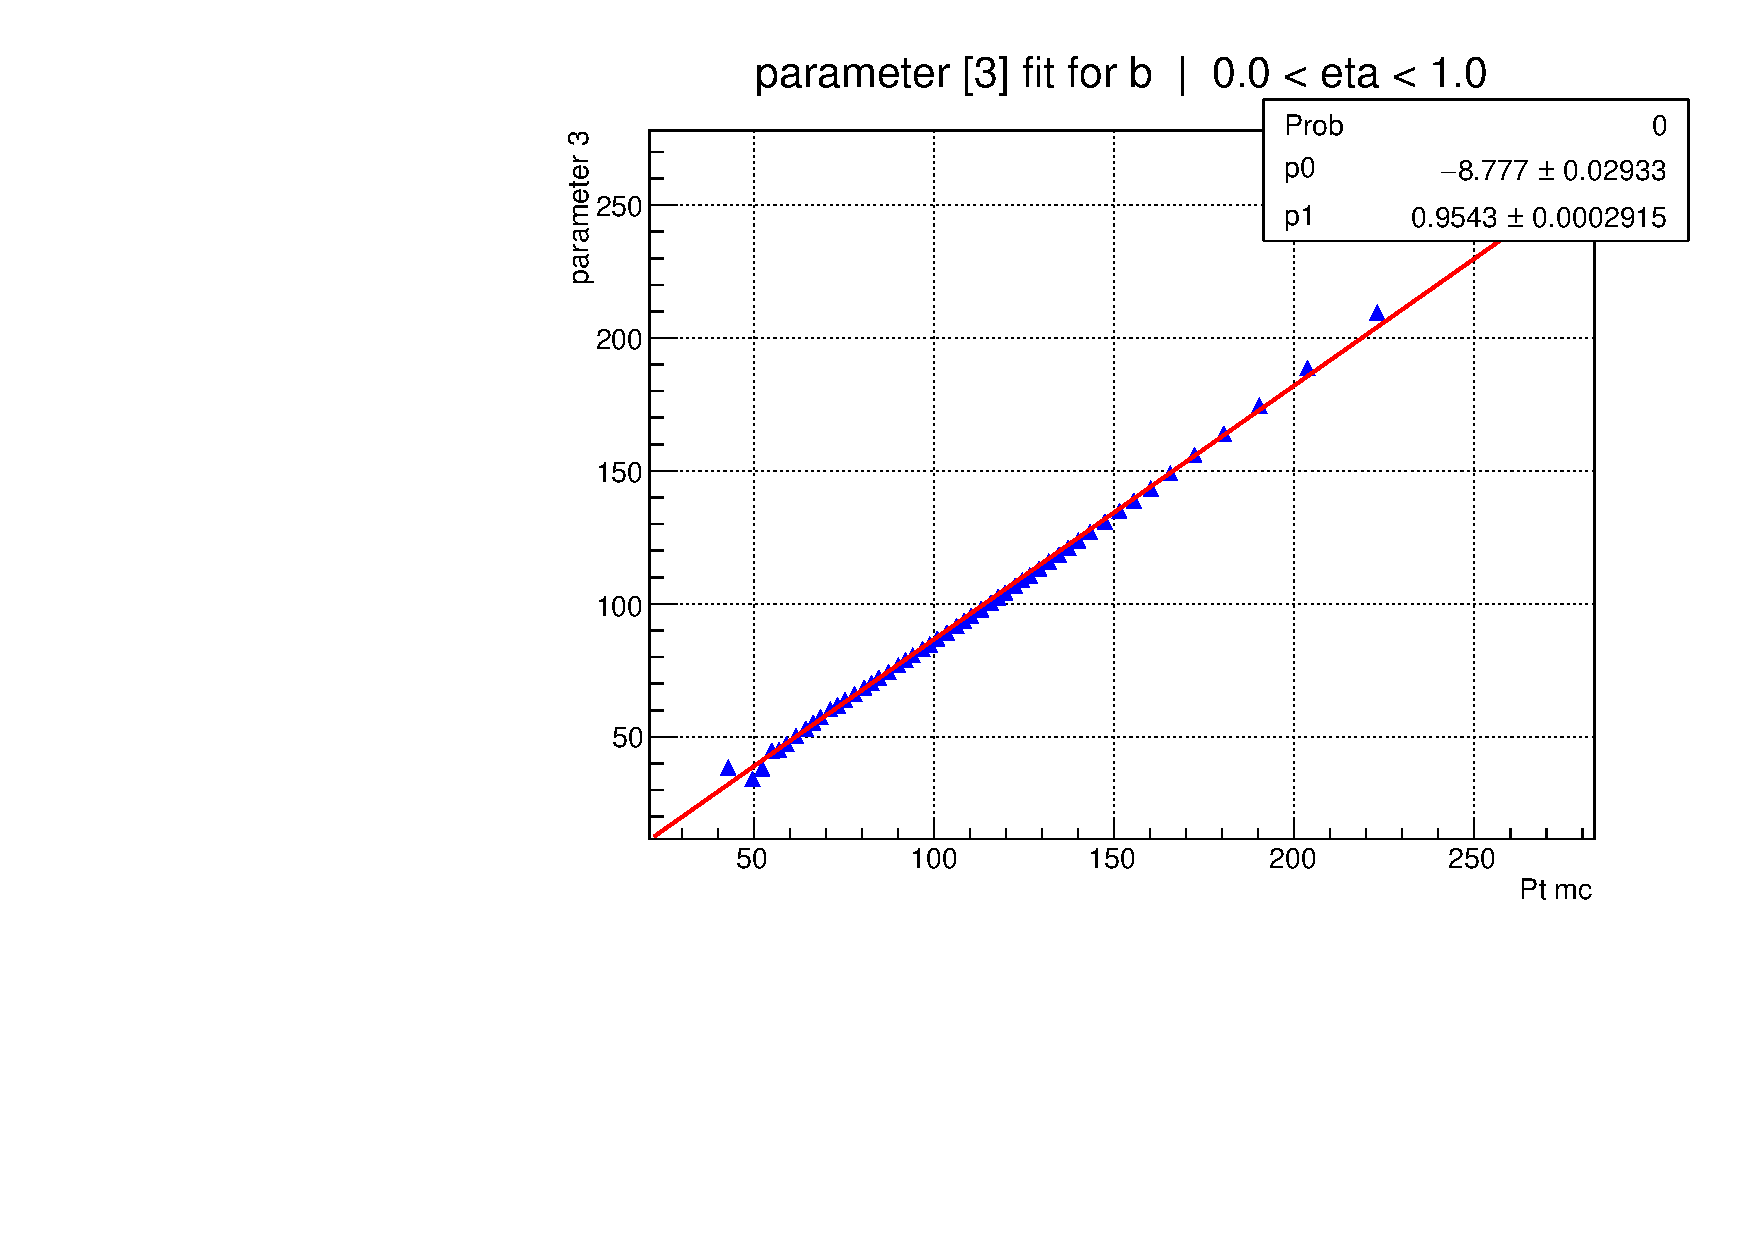
\includegraphics[width = 0.5\textwidth]{figures/transfer/par3-b-eta0.pdf}}
\subfloat[Fit of~$p_4$.]{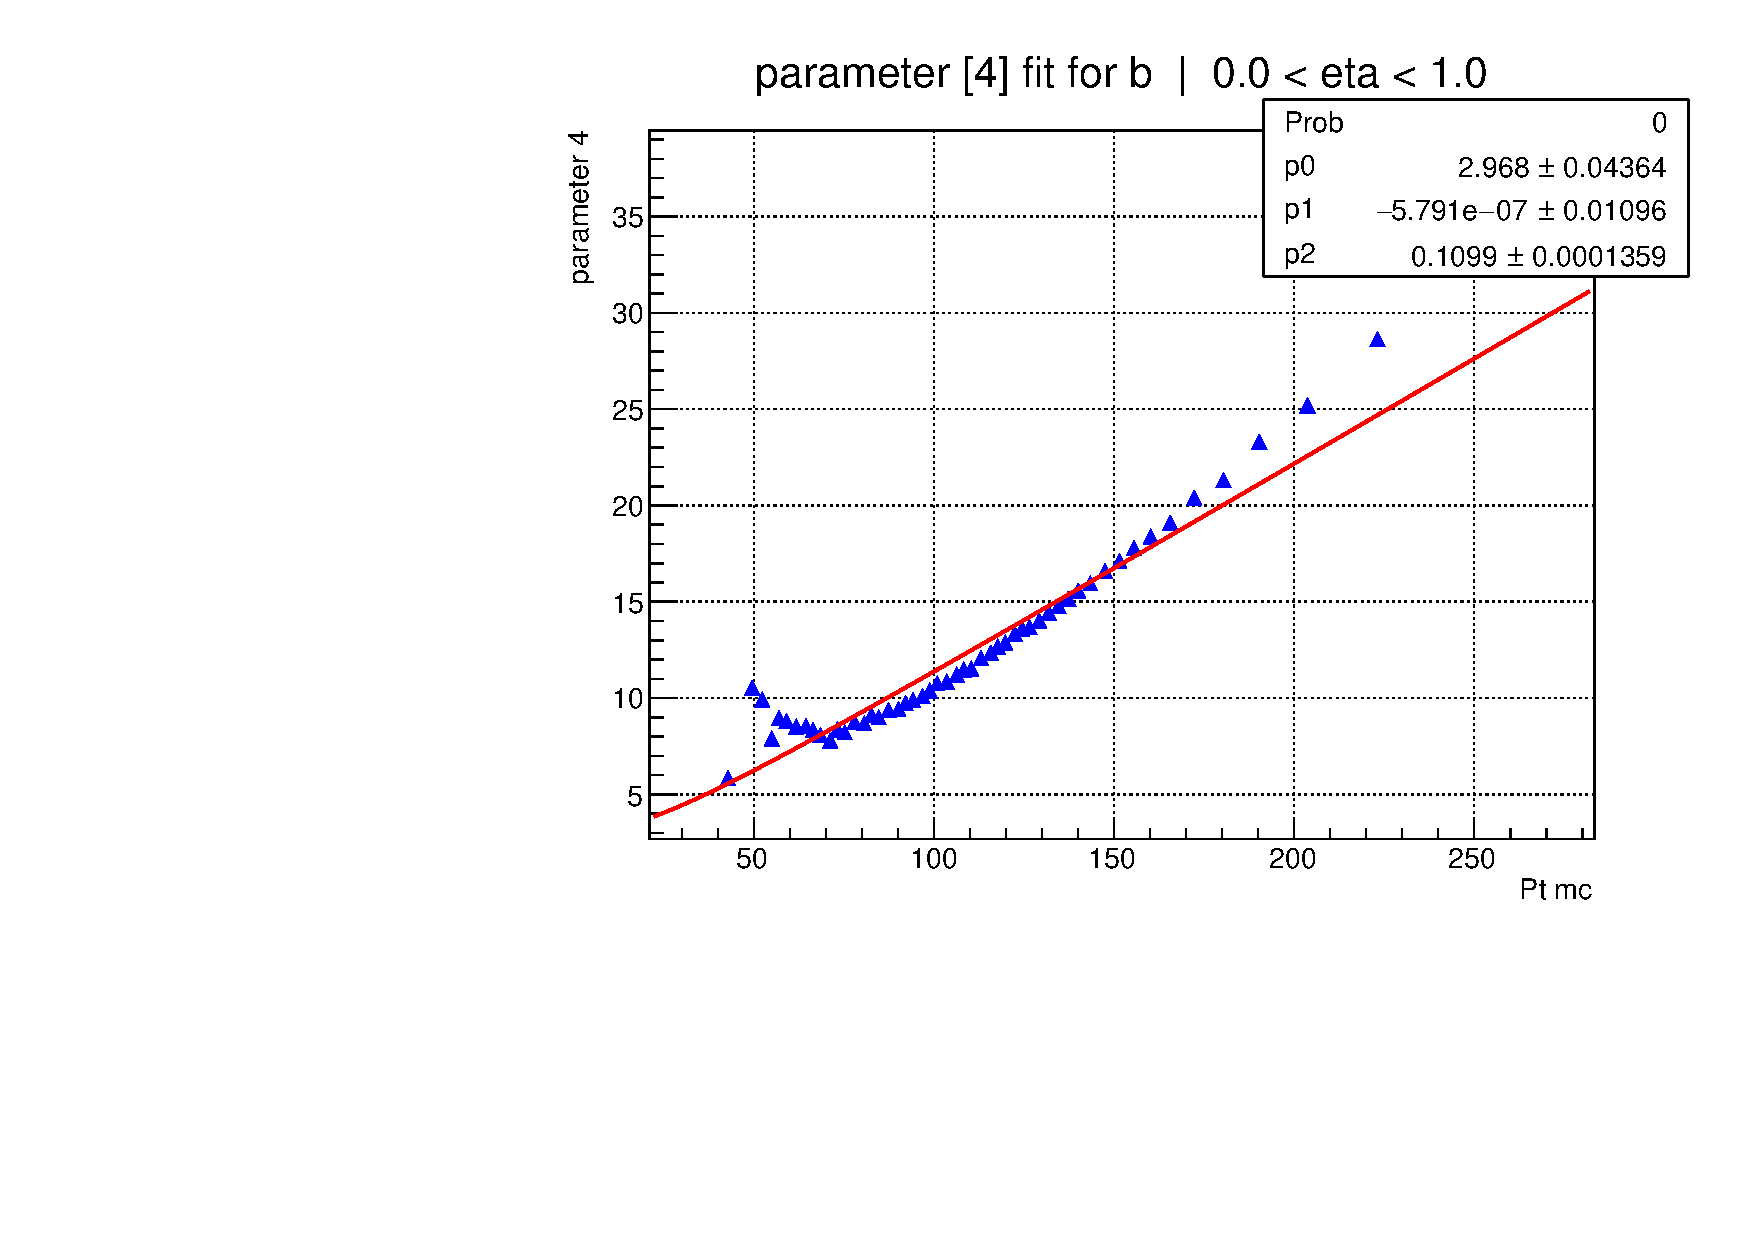
\includegraphics[width = 0.5\textwidth]{figures/transfer/par4-b-eta0.pdf}} \\
\caption[The dependence of the transfer function fit parameters on jet kinematics]{The fitted parameters of the function~\cref{eq:double_gaussian}~in the form of~$p_n(\ptgen|\eta_{q},\mathrm{f})$. Overall, we see a sufficiently flexible description of the parameters derived in the individual fits (blue) by the polynomial fit (red). The bias in~$p_4$ near~$\ptgen \simeq 50$ GeV is due to the underlying double Gaussian fit not being able to accommodate the jets that fall below the~$p_T$ threshold when reconstructed with the experimental resolution and does not affect the MEM significantly. The fits are derived using~\ttbar+jets simulation.}
\label{fig:transfer_acrossbin}
\end{centering}
\end{figure}


As we are considering both SL and DL~\ttH~decays, the reconstruction resolution of~\MET~has to be taken into account via a transfer function. We model it via a Gaussian with a resolution~$\sigma_{MET}^2 = 30\GeV$, which is of similar magnitude to detector resolution and does not affect the results significantly.
It is possible to evaluate the covariance matrix of~\MET~on an event-by-event basis and thus take into account the correlation between the~$\MET_x$ and~$\MET_y$ components in the MEM~\cite{2011JInst...6.9001C}. This leads to the full~\MET~transfer function in the form of a  multivariate Gaussian

\begin{equation}
W_{\MET}(\vec{\rho}_T | \sum_k \vec{p}_k) = \frac{1}{2\pi |\Sigma|^{1/2}} \exp \biggl[ -\frac{1}{2} (\vec{\rho}_T - \sum_k \vec{p}_k)^T \Sigma^{-1} (\vec{\rho}_T - \sum_k \vec{p}_k)\biggr],
\end{equation}
where we currently have assumed~$\Sigma = \sigma_{\MET} \mathbf{I}$ as a first approximation.

\subsection{Lost quarks}
\label{sec:lost_quarks}

In Run II, we have extended the MEM to deal with scenarios where one or more of the quarks from the underlying~$pp \rightarrow~\ttH(\rightarrow \bb),\ttbb$ processes is not reconstructed due to either being out of the geometrical detector acceptance~$|\eta_j| > \eta_{\mathrm{cut}}$ or due to hadronising into a jet that is below an experimental threshold~$E_j < E_{\mathrm{cut}}$.
To achieve this, we formally extend the space of observables~$\vec{y} \rightarrow \vec{y}' = (\vec{y}, (E_q, \vec{e}_q)_{q \in \mathrm{lost}})$ and the per-event matrix element probability

\begin{equation}
P(\vec{y}) \rightarrow P'(\vec{y}') = \frac{1}{\sigma'} \frac{\mathrm{d} \sigma_i}{\mathrm{d}\vec{y} \prod_{q\in\mathrm{lost}} \mathrm{d}E_j \mathrm{d}\vec{e}_j}
\end{equation}
and integrate out the unobserved quantities:

\begin{equation}
P(\vec{y}) = \int_{\mathcal{A}'} \bigl[ \prod_{q \in \mathrm{lost}} \mathrm{d}E_q \mathrm{d}\vec{e}_q \bigr] P'(\vec{y}').
\end{equation}
As the quark can be out of acceptance either due to failing the geometrical acceptance in $\eta$ or falling below the energy threshold, the integral over the lost quarks simplifies to

\begin{equation}
P(\vec{y}) = \int \dots \times \prod_{q\in\mathrm{lost}} \biggl[ \int_{|\eta_q| \leq \eta_{\mathrm{cut}}} \mathrm{d}\Omega_q \epsilon(E_q, \eta_q) \dots + \int_{|\eta_q| > \eta_{\mathrm{cut}}} \mathrm{d}\Omega_q \dots \biggr] \times \dots
\end{equation}
where~$\epsilon(E_q, \eta_q)$ is the probability for a quark of energy~$E_q$ at a pseudo-rapidity~$\eta_q$ to hadronize to a jet below the energy threshold~$E_{\mathrm{cut}}(\eta_q)$ and thus fail to be reconstructed:

\begin{equation}
\epsilon(E_q, \eta_q) = \int_0^{E_{\mathrm{cut}}(\eta_q)} \mathrm{d}E_j W(E_j | E_q).
\end{equation}
This means that for every lost quark, we add 2 integration variables through~$\mathrm{d}\Omega_q$, as well as an extra combination of choosing which of the quarks did not produce a jet. The flexibility afforded by this technique, which makes the MEM applicable for cases where we may not always reconstruct the exact multi-particle final state, thus comes at a computational cost which is evaluated in~\cref{sec:mem_computational}.

\subsection{Treatment of QCD radiation}
\label{sec:mem_radiation}

The MEM as formulated above does not account for QCD radiation, which at the LHC can be substantial~\cite{Alwall:2010cq}. In particular, we estimate using simulation that the ratio between 7 and 6 reconstructed jets is~$N_{7\mathrm{jet}}/N_{6\mathrm{jet}} \simeq 0.5$ for~\ttHbb, whereas the hard interaction produces only 6 partons at LO. Therefore there is a substantial fraction of events with more jets than is naively required for the MEM and we need to either define a selection among those jets or model them. Additionally, ISR that is not reconstructed as jets also affects the kinematics of the event with an unknown component in the final momentum balance. We have implemented and compared several alternative techniques that extend the MEM to final states with additional jets arising from radiation.

First, to deal with unreconstructed ISR, we note that momentum balance can be restored by performing a Lorentz boost with~$\beta(\vec{p}_k) = (\sum_k p_{k,x}, \sum_k p_{k,y}, \beta_z)$ in the transverse plane, such that a Born-like configuration with a null transverse momentum is achieved. The longitudinal component~$\beta_z$ of the boost is in principle unknown and should be integrated out. However, we find that it can be ignored by setting~$\beta_z = 0$, since it corresponds to different values for gluon fractions~$x_{1,2}$ which are found not to affect the performance of the matrix element significantly. This simple treatment of ISR kinematics is necessary to evaluate the LO matrix element with proper momentum balance, but it does not take into account the dynamics of ISR production nor the properties of QCD radiation in general.

A possible step forward would be to use additional matrix elements with more final state partons to take into account extra jets. In particular, for events with one extra jet, we can use the~$\mathrm{pp} \rightarrow~\ttHbb~+ \mathrm{g}$ matrix element with an additional gluon. For a semileptonic top decay, we would thus have 7 final state partons that need to be matched to 7 jets. This approach has the advantage of not making the assumption that the extra jet arises necessarily from ISR, but is instead a full treatment of the~$2 \rightarrow 7$ scattering with perturbation theory. However, the additional computational complexity is significant, especially if (anti)quark diagrams are included in addition to the gluon.

Sudakov reweighting allows us to approximate the effects of ISR in the scattering amplitude in terms of splitting functions derived from QCD. At detector level, the Sudakov factor is approximated by a log-normal transfer function of the form

\begin{equation}
W(p_T) = \frac{1}{\sqrt{2\pi} \sigma p_T} \exp \biggl[ \frac{-(\ln{p_T/1~\mathrm{GeV}} - \mu)^2}{2\sigma^2}\biggr]
\end{equation}
that approximates the probability of the parton-level transverse momentum~$p_T$ resulting in an observed recoil~$\rho_T$ below an experimental threshold~$\rho_{T,0} < 30~\mathrm{GeV}$, taking into account detector resolution. Here the the values~$\mu = 4.1$ and~$\sigma = 1.35$ are estimated from MC simulation and the unknown momentum ISR momentum~$p_T$ is integrated out. We have implemented this empirical factor and compared it with the nominal LO MEM, however, we have seen that the changes are very small and compatible with MC statistical uncertainties. 

In case a significant missing transverse momentum is observed in the event, a separate double-Gaussian transfer function would be appropriate in the Sudakov factor. However, since we independently have to consider a transfer function for the MET due to the presence of neutrinos, the modelling of ISR recoil can be absorbed in the MET recoil transfer function, as explained in~\cref{sec:transfer_functions}.

\subsection{Event interpretations}
\label{sec:event_interpretation}

The scattering amplitude~$|\mathcal{M}_{\vec{\theta}}|$ depends on the assumed process~$\mathcal{H}$ and the interpretation of the event~$\mathcal{C}$. Various interpretations are possible, depending on the observed multiplicity of charged leptons and jets. First, the number of charged leptons fixes the choice of the top decay amplitudes between the semileptonic, dileptonic or all-hadronic. This in turn determines the number of quarks in the final state. Depending on the nature and number of the observed jets, we consider 4 classes of event interpretations:

\begin{itemize}
\item \textbf{Fully reconstructed events}: In this case~$N_{\mathrm{jets}} = N_{\mathrm{quarks}}$, such that each each quark is associated with a jet. This is the standard case.
\item \textbf{Over-reconstructed events}: If~$N_{\mathrm{jets}} > N_{\mathrm{quarks}}$, we may choose up to~$N_{\mathrm{quarks}}$ jets out of the set of reconstructed jets, such that each quark is associated with a jet and the left-over jets are ignored. In doing this, we sum over the possible choice of jets using the combinatorial approach of the MEM.
\item \textbf{Over-reconstructed events with an ISR interpretation}: If~$N_{\mathrm{jets}} = N_{\mathrm{quarks}} + 1$, we may act as above, but choose to interpret the extra jet as arising from gluon radiation in the initial state using the LO diagrams~$\ttH + \mathrm{g}$ and ~$\ttbb + \mathrm{g}$ in a full MEM approach by extending the reconstructed phase space~$\vec{y}$. Due to the higher complexity of the involved diagrams, this approach is computationally more costly than the above, but includes information on the dynamics and kinematics of the additional jet.
\item \textbf{Partially-reconstructed events}: In case~$N_{\mathrm{jets}} < N_{\mathrm{quarks}}$, we treat a number of quarks as lost and integrate over their directions as described in~\cref{sec:lost_quarks}. This allows the MEM to be used as a discriminator on a wider range of events, but we may also apply this hypothesis in case we suspect some jets may be mismeasured and not correspond to the underlying hard interaction, thus integrating them out.
\end{itemize}

In the most general case, we could evaluate all possible event interpretations and use them as a combined event discriminator that makes maximal use of kinematics and the prior probabilities for each hypothesis. However, this is computationally prohibitive, requiring many numerical integrals per event, with each hypothesis taking~$\mathcal{O}(10^1)\dots \mathcal{O}(10^3)$ seconds on a modern CPU. Therefore, it is necessary to restrict the interpretation space using MC simulation, comparing the expected performance of various interpretation strategies and choosing one providing an acceptable trade-off between discriminator performance and computational cost. We list the interpretations that were considered in~\cref{tab:event_interpretation_list}.

\begin{table}[h!]
\begin{center}
\begin{tabular}{c|ccc}
\hline
interpretation & bottom quarks & light quarks & description \\
\hline
SL~$2_{\mathrm{W}} 2_{\mathrm{h}} 2_{\mathrm{t}}$ & 4 & 2 & fully-reconstructed semileptonic \\
SL~$1_{\mathrm{W}} 2_{\mathrm{h}} 2_{\mathrm{t}}$ & 4 & 1 &~$(l \nu_{l}' \mathrm{b})_{\mathrm{t}} (\cancel{\mathrm{q}} \mathrm{q}' \bar{\mathrm{b}})_{\bar{\mathrm{t}}} (\mathrm{b} \bar{\mathrm{b}})_{\mathrm{h}}$ \\
SL~$0_{\mathrm{W}} 2_{\mathrm{h}} 2_{\mathrm{t}}$ & 4 & 0 &~$(l \nu_{l}' \mathrm{b})_{\mathrm{t}} (\cancel{\mathrm{q}} \cancel{\mathrm{q}'} \bar{\mathrm{b}})_{\bar{\mathrm{t}}} (\mathrm{b} \bar{\mathrm{b}})_{\mathrm{h}}$ \\
SL~$2_{\mathrm{W}} 2_{\mathrm{h}} 2_{\mathrm{t}}+1\mathrm{g}$ & 4 & 3 & fully-reconstructed, additional ISR gluon \\
%SL~$2_{\mathrm{W}} 1_{\mathrm{h}} 2_{\mathrm{t}}$ & 3 & 2 &~$(l \nu_{l}' \mathrm{b})_{\mathrm{t}} (\mathrm{q} \mathrm{q}' \bar{\mathrm{b}})_{\bar{\mathrm{t}}} (\cancel{\mathrm{b}} \bar{\mathrm{b}})_{\mathrm{h}}$ \\
%SL~$2_{\mathrm{W}} 2_{\mathrm{h}} 1_{\mathrm{t}}$ & 3 & 2 &~$(l \nu_{l}' \mathrm{b})_{\mathrm{t}} (\mathrm{q} \mathrm{q}' \cancel{\bar{\mathrm{b}}})_{\bar{\mathrm{t}}} (\mathrm{b} \bar{\mathrm{b}})_{\mathrm{h}}$ \\
\hline
DL~$2_{\mathrm{h}} 2_{\mathrm{t}}$ & 4 & 0 & fully-reconstructed dileptonic \\
%DL~$1_{\mathrm{h}} 2_{\mathrm{t}}$ & 3 & 0 &~$(l \nu_{l}' \mathrm{b})_{\mathrm{t}} (l \nu_{l}' \bar{\mathrm{b}})_{\bar{\mathrm{t}}} (\cancel{\mathrm{b}} \bar{\mathrm{b}})_{\mathrm{h}}$ \\
%DL~$2_{\mathrm{h}} 1_{\mathrm{t}}$ & 3 & 0 &~$(l \nu_{l}' \cancel{\mathrm{b}})_{\mathrm{t}} (l \nu_{l}' \bar{\mathrm{b}})_{\bar{\mathrm{t}}} (\mathrm{b} \bar{\mathrm{b}})_{\mathrm{h}}$ \\
\hline
\hline
\end{tabular}
\caption[The MEM event interpretations considered for different final state topologies]{The detailed event interpretations for semileptonic and dileptonic~\ttH~(signal) and~\ttbb~(background) events. In the semileptonic channel, we consider cases where up to 2 light quarks may be lost. The minimum number of jets required for a hypothesis is the sum of the number of quarks. For the SL~$1_{\mathrm{W}} 2_{\mathrm{h}} 2_{\mathrm{t}}$ hypothesis the direction and energy of one of the light quarks is integrated out, denoted by $\cancel{\mathrm{q}}$. For the fully-reconstructed semileptonic case with 7 jets, we also consider the ISR-modified interpretation.}
\label{tab:event_interpretation_list}
\end{center}
\end{table}

We use a number of strategies to restrict the number of combinations that need to be considered in the transfer function~\cref{eq:tf_combination_sum}. 

\begin{itemize}
\item As we are dealing with up to 2 oppositely-charged leptons, we can neglect the small effect of charge confusion and assume the leptons are identified perfectly in case of a dileptonic event.
\item We assume that the efficiency of correctly b~tagging jets arising from bottom quarks (mistagging light jets) is sufficiently high (low) that we find bottom quark (light quark) candidates only among b~tagged (untagged) jets.
\item If we have more than 3 candidates for the light quarks, we select the 3 that are most compatible with a~$\mathrm{W} \rightarrow \mathrm{q}\mathrm{q}'$ decay according to invariant mass.
\item We take note that the scattering amplitude~$|\mathcal{M}|^2$ is symmetric under charge exchange, therefore, we only compute the scattering amplitude with only one combination corresponding to a particular charge assignment of quarks.
\end{itemize}
The jets are assumed to be b~tagged or untagged by choosing the set of jets that is most compatible with arising from a 4 b~quark hypothesis using a likelihood ratio based on jet b~discriminators, as will be explained further in~\cref{sec:object_id_btag}. Overall, the number of transfer function combinations that are required for each hypothesis in the categories we use is show in~\cref{tab:category_combinations}. These assumptions are found not to reduce the performance of the MEM significantly, but they decrease the number of combinations (and thus computational burden) by an order of magnitude, as seen on figure~\cref{fig:mem_assumptions}. In fact, we find that being more strict with the assumptions can help boost the discriminating power of the MEM, as it helps to separate the more probable combinations from the less probable ones in the combination sum in~\cref{eq:tf_combination_sum}.

\begin{table}[h!]
\begin{center}
\begin{tabular}{c|ccccc}
\hline
interpretation& 8+ jets & 7 jets & 6 jets & 5 jets & 4 jets \\
\hline
SL~$2_{\mathrm{W}} 2_{\mathrm{h}} 2_{\mathrm{t}}$ & 72/36 & 36 & 12 & - & - \\
SL~$1_{\mathrm{W}} 2_{\mathrm{h}} 2_{\mathrm{t}}$ & - & - & - & 12 & -\\
SL~$0_{\mathrm{W}} 2_{\mathrm{h}} 2_{\mathrm{t}}$ & - & - & - & - & 12 \\
SL~$2_{\mathrm{W}} 2_{\mathrm{h}} 2_{\mathrm{t}}+1\mathrm{g}$ & 72/36 & 36 & - & - & - \\
\hline
DL~$2_{\mathrm{h}} 2_{\mathrm{t}}$ & 12 & 12 & 12 & 12 & 12 \\
\hline
\hline
\end{tabular}
\caption[The number of MEM combinations in different categories]{The number of MEM combinations in associating quarks to jet for various MEM categories. In SL events with 7 or more jets, we choose up to 4 candidates based on invariant mass among the light jets for the W-boson reconstruction, in order to prevent a combinatorial explosion for events with a very high jet multiplicity. In DL events, we always choose exactly 4 candidates for the b~quarks.}
\label{tab:category_combinations}
\end{center}
\end{table}

\begin{figure}
\begin{centering}
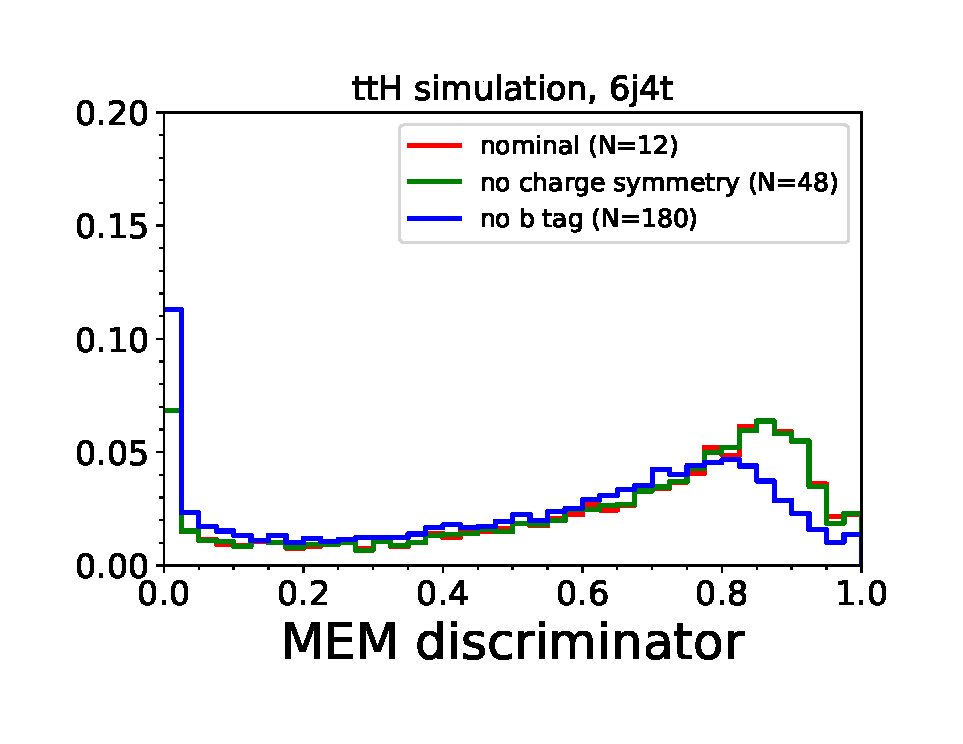
\includegraphics[width=0.5\textwidth]{figures/mem/mem_assumptions.pdf}
\caption[The effect of combinations assumptions in the MEM]{The effect of combination assumptions in the MEM discriminator based on~\ttHbb~simulation. We compare the nominal case (red), where the combinations are restricted according to b~tagging and assuming a single charge assignment, with the case where the charge assignment restriction is removed (green, 48 combinations) and the case where the b~tagging restriction is removed (blue, 180 combinations). We see that the charge assignment has negligible effect on the overall discriminator shape, whereas the b~tagging significantly increases number of permutations and thus reduces the discriminating power of the MEM.}
\label{fig:mem_assumptions}
\end{centering}
\end{figure}

\subsection{Integration}
\label{sec:mem_integration}

The MEM is implemented as a dedicated code in C++, relying on the~\texttt{OpenLoops} library~\cite{Cascioli:2011va} interfaced via C++ for the evaluation of the hard scattering amplitude. The~\texttt{ROOT} package~\cite{Brun:1997pa} is used for numerical Lorentz algebra and~\texttt{CLING}~\cite{Vasilev:2012ev} for interfacing the code to Python with the rest of the analysis. The PDFs are evaluated using the~\texttt{cteq66} set via the~\texttt{LHAPDF}~package~\cite{Buckley:2014ana}. The numerical integration routines rely on the~\texttt{VEGAS}~algorithm~\cite{Lepage:1977sw} that uses multiple passes to refine the integration grid, with the maximal number of evaluations tuned for approximately~$\Delta I / I < 2.5 \dots 5\%$ relative numerical accuracy on the integral, suitable for use in a discriminator. We use the~\texttt{CUBA}~package~\cite{Hahn:2004fe} for numerical integration, as it supports vector-valued integrands. The distribution of expected numerical accuracy is shown on~\cref{fig:mem_numerical_accuracy} and illustrates the convergence of the numerical integration. We see that the computational cost is around 1-2 CPU minutes per event including both the signal and background hypotheses and that the numerical integration is accurate to within~$5\%$ on average. Transfer functions can be provided in a flexible parametrisation using \texttt{ROOT}, however, as described in~\cref{sec:mem_optimisation}, we have also provided faster, optimised versions of the Gaussian transfer functions.

In~\cref{sec:mem_implementation} we have expressed the integral~\cref{eq:mem_definition}~in terms of variables which are aligned with the peaks of the integrand. In general, we could integrate over the full allowable range of these variables, however, to improve convergence, we restrict the integration over energies to a symmetric confidence region around the reconstructed energy based on the transfer functions. In particular, we derive the lower~($E_L(E_j,\alpha)$)~and upper~($E_L(E_j,\alpha)$)~integration boundaries for a jet with energy~$E_j$ from

\begin{equation}
\int_{E_L(E_j,\alpha)}^{E_H(E_j,\alpha)} \mathrm{d}E_q W(E_j | E_q) = \alpha
\end{equation}
with~$\alpha = 0.95$ and choose the integration variable~$x_q$ for the quark energy such that~$E_q(x_q) = E_L + x_q (E_H - E_L)$, to restrict the integration into the range~$x\in[0,1]$ as required by the VEGAS algorithm. The integration with respect to the angular variables is performed over the ranges~$\phi \in [-\pi, +\pi]$ and~$\cos{\theta} \in [-1, +1]$.

\subsubsection{VEGAS algorithm}
In computing the full ME scattering amplitude and transfer function convolution of~\cref{eq:mem_definition}, we rely on numerical MC integration for the results. The integral is approximated by a weighted sum over sampled points~$\mathbf{x}_i$ such that

\begin{equation}
I = \int f(\mathbf{x})\ \mathrm{d}\mathbf{x} \simeq \tilde{I} = \frac{1}{N} \sum_{i}^N w_i f(\mathbf{x}_i).
\end{equation}
The variance in the estimation $\tilde{I}$ is given by

$$\mathrm{Var}(\tilde{I}) = \frac{\mathrm{Var}(f)}{N};\ \mathrm{Var}(f) = \frac{1}{N-1} \sum_i^N(f(\mathbf{x}_i) - \langle f \rangle)^2$$
in case $w_i = 1$. Choosing the weights appropriately allows the variance to be reduced, such that for $w_i = \frac{|f(\mathbf{x}_i)|}{\int f \mathrm{d}\mathbf{x}}$, the variance disappears. The VEGAS implementation in CUBA relies on importance sampling, which increases the amount of points where $|f|$ is large, by constructing the weights as a piecewise constant function in the integration hypercube, refined by iteratively increasing the number of integration samples. We use between $\mathcal{O}(10^3)$ and $\mathcal{O}(5 \times 10^4)$ integration points in 5 successive stages. An example of the final VEGAS integration grid is shown on figure~\cref{fig:vegas_grid}, where we see that the integration points are clustered around $\alpha=0.5$, which corresponds to an on-peak quark reconstruction $E_q = E_j$ and somewhat more spread out in the neutrino polar angle. We can see that the peak dimensions are aligned with the integration axes by the construction of the Jacobian, which is necessary for efficient integral evaluation via VEGAS.

\begin{figure}[ht]
\begin{centering}
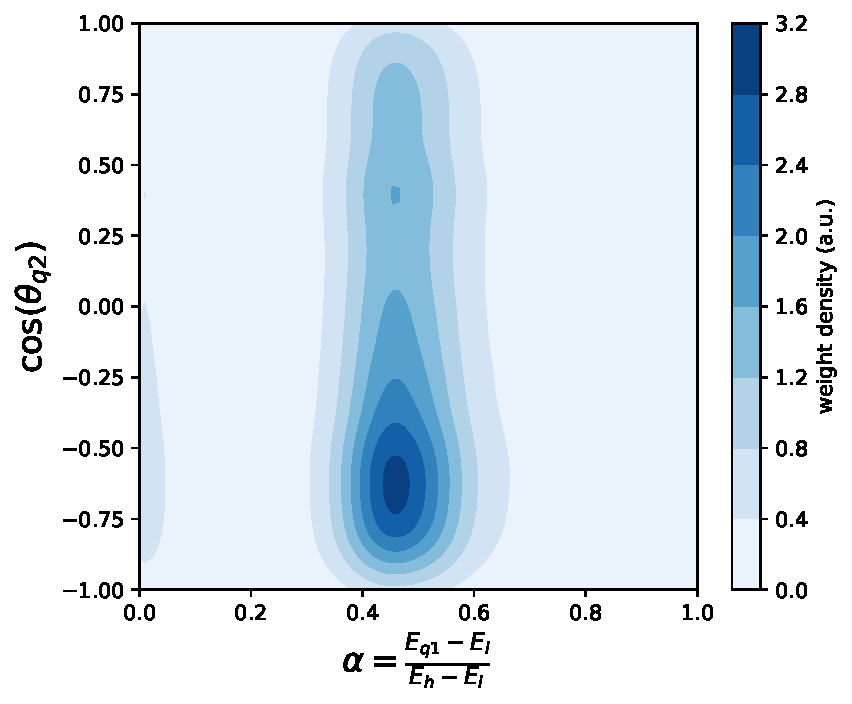
\includegraphics[width = 0.4\textwidth]{figures/mem/vegas_grid.pdf}
\caption[VEGAS grid example]{An example of the VEGAS integration weights in the plane defined by the light quark energy fraction and neutrino polar angle.}
\label{fig:vegas_grid}
\end{centering}
\end{figure}

\begin{figure}
\begin{centering}
\subfloat[Integration time of the MEM.]{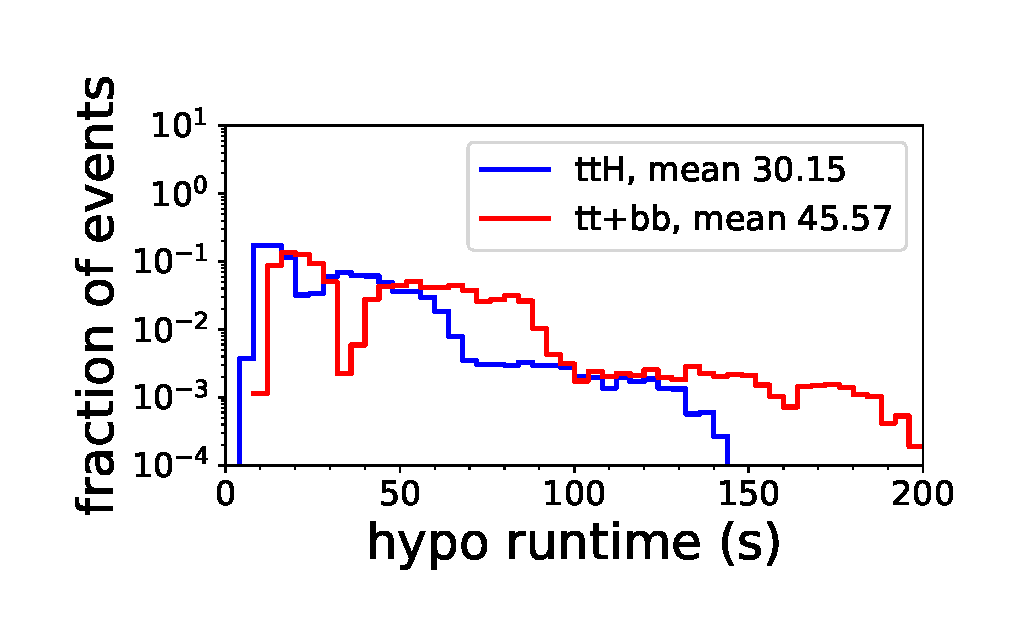
\includegraphics[width = 0.5\linewidth]{figures/mem/mem_time.pdf}} 
\subfloat[Numerical uncertainty of the MEM]{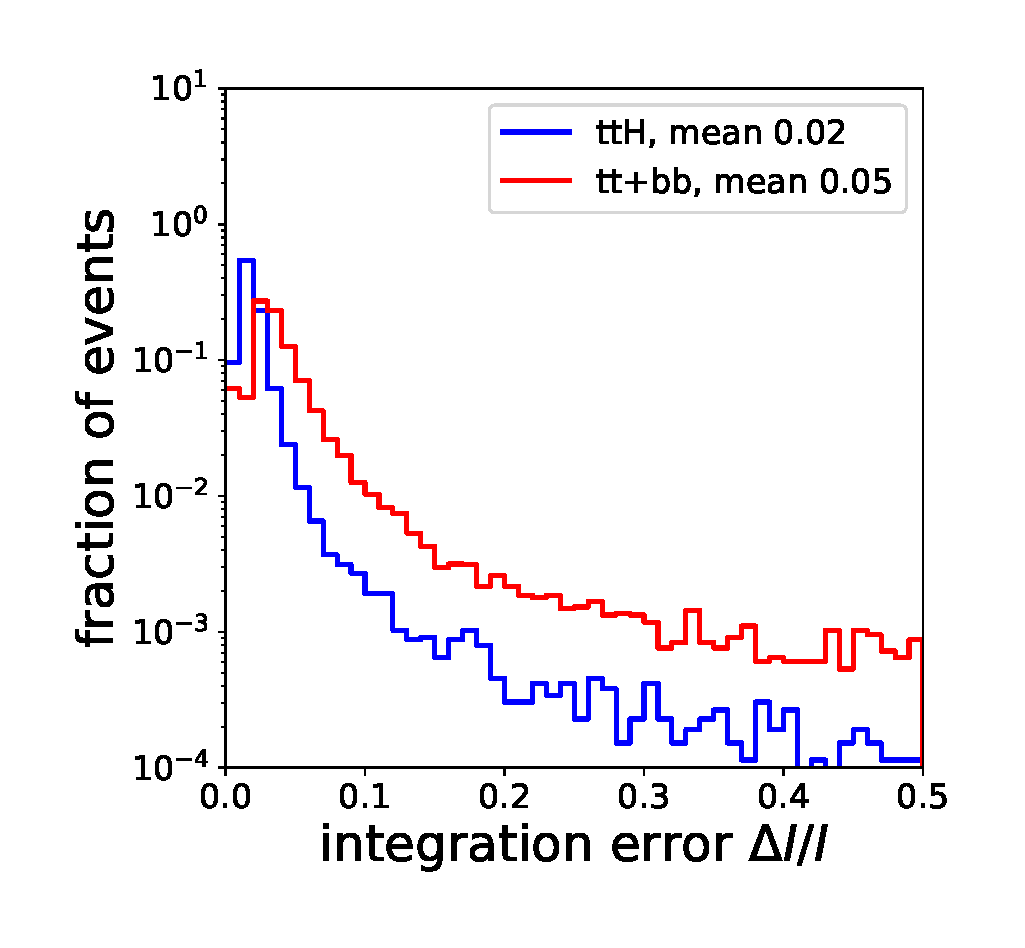
\includegraphics[width = 0.5\linewidth]{figures/mem/mem_error.pdf}}\\
\caption[The MEM integration time.]{The integration time (\textbf{a}) and uncertainty resulting from numerical integration (\textbf{b}) of the MEM discriminator for the fully reconstructed hypothesis. In general, we see that the average time to compute the MEM discriminator is below 1 minute for both the signal and background hypotheses, with a significant spread due to the varying number of jets in events and thus the number of combinations that need to be considered. The background hypothesis is significantly more computationally expensive, due to the complexity of the~\ttbb~diagrams compared to~\ttHbb. The numerical uncertainty is below~$5\%$ on average for both the signal and background hypotheses, with a larger spread for the background hypothesis.}
\label{fig:mem_numerical_accuracy}
\end{centering}
\end{figure}

For the SL~$2_{\mathrm{W}} 2_{\mathrm{h}} 2_{\mathrm{t}}$~signal hypothesis, the integration is carried over 4 variables: the top-associated light quark energy $E_{q_t}$, the neutrino directions $\cos{\theta_\nu}$ and $\cos{\phi_\nu}$ and the energy of the Higgs-associated b~quark $E_{b_H}$. An additional axis is introduced for the~\ttbb~hypothesis, integrating over the energy of the second b~quark not associated to top quark decay~$(E_{\bar{b}_H}$). The addition of each lost quark adds an additional energy integration, such that for the~SL~$0_{\mathrm{W}} 2_{\mathrm{h}} 2_{\mathrm{t}}$~hypothesis, we have 6 integration dimensions for the~\ttHbb~hypothesis and 7 for the~\ttbb~hypothesis. In the dileptonic channel, the DL~$2_{\mathrm{h}} 2_{\mathrm{t}}$~signal hypothesis has 5 integration variables: 2 angles per neutrino, plus the energy of one of the Higgs-associated b-quarks~$E_{b_H}$.

\subsection{Profiling and optimisation}
\label{sec:mem_optimisation}

In order to optimise the MEM code, we have used the~\texttt{igprof}~sampling profiler~\cite{Eulisse:2005zz,Tuura:2008zza} to analyse the computational budget spent in various subroutines of the code. In general, we find    
that the overwhelming majority of time is spent within the integrand, out of which about 40\% is spent computing the transfer functions, 35\%~is~spent evaluating the scattering amplitude of the hard process, 10\%~on~computing the PDFs and about~10\%~on~manipulating the phase space volume. The evaluation of the transfer functions at a single phase space point is about an order of magnitude faster than the scattering amplitude. In order to achieve this ratio, we implemented the transfer functions explicitly as optimised C++ functions, instead of relying on a more generic approach using symbolic functions supported in ROOT. Additionally, as a large part of time optimising the integration grid is spent in evaluating the exponential tails of the transfer function, we have used a piecewise exponential function that is suppressed far in the tails.

Currently, the MEM algorithm as implemented here can only be run on standard x86 CPU architectures. Although it has been shown that GPUs may offer strong parallelization benefits in evaluating the integral, it would be necessary to completely port and optimise the~\texttt{OpenLoops} toolset, or another ME library, on the GPU in a significant engineering effort~\cite{Schouten:2014yza}, furthermore, GPU clusters are currently not commonplace in the Worldwide LHC Grid (WLCG), limiting the applicability of the code. However, in the future, as massively parallelized resources and automatic code translation tools become more widely available, the phase space integration could benefit significantly from parallel resources.

\subsection{Computational budget}
\label{sec:mem_computational}
In this section, we present a feasibility estimation on using the MEM in a Run II analysis. This is necessary in order to predict the amount of computing resources that will be required. The computing time depends strongly on the number of combinations and integration variables needed for a given interpretation and event topology, as well as the total number of MC simulated events that are needed for the analysis. In~\cref{tab:mem_cpu_budget}, we show the required CPU budget for evaluating the MEM on various event topologies. Based on this, we identify the MEM interpretations to apply on a given event topology. In particular, we see that the treatment of the additional gluon radiation in the MEM diagram increases the computational cost by about a factor of 5, mainly from the~\ttbb~amplitude. Furthermore, we find that computing the MEM with a hypothesis that considers all the reconstructed jets provides the best trade-off between performance and computing cost.

\begin{table}[h!]
\begin{center}
\begin{tabular}{c|ccccc}
\hline
method & time~\ttH~(s) & time~\ttbb~(s) & ROC AUC &~$\epsilon_{\mathrm{bkg}}$ & total (h) / 1k \\
\hline
SL,~$\ge7$jet,~$2_{\mathrm{W}} 2_{\mathrm{h}} 2_{\mathrm{t}}$ &~$45.8 \pm 18.9$ &~$69.4 \pm 26.1$ &~$0.315$ &~$0.232$ &~$32.00$\\
SL,~$\ge7$jet,~$2_{\mathrm{W}} 2_{\mathrm{h}} 2_{\mathrm{t}} 1_{\mathrm{g}}$ &~$71.7 \pm 27.1$ &~$471.7 \pm 50.6$ &~$0.317$ &~$0.233$ &~$150.94$\\
SL,~$\ge6$jet,~$2_{\mathrm{W}} 2_{\mathrm{h}} 2_{\mathrm{t}}$ &~$30.2 \pm 21.0$ &~$45.4 \pm 30.9$ &~$0.321$ &~$0.233$ &~$21.00$\\
SL,~$\ge6$jet,~$1_{\mathrm{W}} 2_{\mathrm{h}} 2_{\mathrm{t}}$ &~$64.8 \pm 22.7$ &~$101.1 \pm 33.0$ &~$0.307$ &~$0.210$ &~$46.07$\\
SL,~$\ge6$jet,~$0_{\mathrm{W}} 2_{\mathrm{h}} 2_{\mathrm{t}}$ &~$83.9 \pm 20.4$ &~$136.3 \pm 28.9$ &~$0.294$ &~$0.218$ &~$61.16$\\
SL, 5jet,~$1_{\mathrm{W}} 2_{\mathrm{h}} 2_{\mathrm{t}}$ &~$25.4 \pm 7.1$ &~$39.9 \pm 9.6$ &~$0.293$ &~$0.198$ &~$18.13$\\
SL, 5jet,~$0_{\mathrm{W}} 2_{\mathrm{h}} 2_{\mathrm{t}}$ &~$84.7 \pm 20.3$ &~$136.9 \pm 28.9$ &~$0.291$ &~$0.217$ &~$61.56$\\
SL, 4jet,~$0_{\mathrm{W}} 2_{\mathrm{h}} 2_{\mathrm{t}}$ &~$84.3 \pm 20.7$ &~$136.0 \pm 29.2$ &~$0.333$ &~$0.275$ &~$61.21$\\
DL,~$\ge4$jet,~$0_{\mathrm{W}} 2_{\mathrm{h}} 2_{\mathrm{t}}$ &~$55.7 \pm 13.7$ &~$90.4 \pm 19.3$ &~$0.223$ &~$0.124$ &~$40.58$\\
\hline
\hline
\end{tabular}
\caption[The CPU budget and separation of the MEM in different categories]{The CPU budget and separation power of the MEM in the SL channel using various event interpretations. We show the time required to evaluate the signal and background hypotheses, the receiver operating characteristic (ROC) area under curve (AUC), the efficiency of background at a signal efficiency of~$50\%$ ($\epsilon_{\mathrm{bkg}}$) and the total time required to compute the MEM discriminator for 1000 events.}
\end{center}
\label{tab:mem_cpu_budget}
\end{table}

\subsection{Propagating uncertainties}
\label{sec:mem_uncertainties}

When using the MEM in a realistic experimental analysis, we need to evaluate the effect of systematic uncertainties on the MEM. In general, uncertainties modify the observables~$\vec{y} \rightarrow \vec{y}^*$, for example the jet energies may be modified by uncertainties in the jet energy scale calibration. The naive approach to estimate the sensitivity of the discriminator would be to recompute the MEM discriminator weights~$P(\vec{y}) \rightarrow P(\vec{y}^*)$. However, this turns out to be impractical, since the number of individual variations that need to be considered can easily reach~$\mathcal{O}(10^2)$ and it is not realistic or practical to expend two orders of magnitude more computational resources.

In order to reduce the computing time, we have developed an approximation for the effect of jet energy scale uncertainties using the analytical form of the MEM. We first note that the variations are generally small, such that~$\vec{y}^* \simeq \vec{y} + \delta \vec{y}$. Therefore, the numerical integration described in section~\cref{sec:mem_implementation} would be performed on almost the same phase space, with a very similar integration grid.

Furthermore, we see from~\cref{eq:mem_definition} that the observables enter the definition of the MEM probability primarily through the transfer functions~$W(\vec{y} | \vec{p})$ and affect the integration volume only secondarily. The most computationally costly part in the integrand is the evaluation of the LO scattering amplitudes for the hard process. Therefore, if we can promote the integrand to a vector-valued quantity, such that

\begin{equation}
|\mathcal{M}(\vec{p})|^2 W(\vec{y} | \vec{p}) \rightarrow |\mathcal{M}(\vec{p})|^2  \begin{pmatrix}
  W(\vec{y} | \vec{p}) \\
  W(\vec{y} + \delta \vec{y}_1 | \vec{p}) \\
  \dots \\
  W(\vec{y} + \delta \vec{y}_n | \vec{p})
 \end{pmatrix}
\end{equation}
and the integration of the nominal and variated weight can be performed in a single pass using a a grid optimised for the whole integration. We have tested this approach by comparing the variation evaluated using vector integration to the full computation with shifted inputs, showing the comparison of the full variation and the approximation on~\cref{fig:jes_variation}. As we wish to estimate the sensitivity of the analysis to this uncertainty, it is sufficient if the approximated variation has the same magnitude and direction as the true variation.

\begin{figure}[ht]
\begin{centering}
\subfloat[Up-variation]{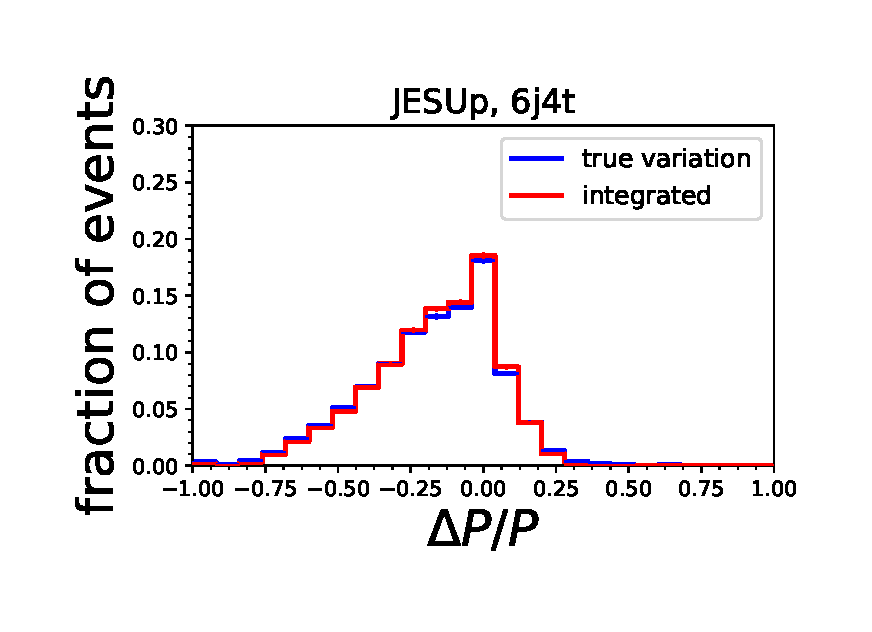
\includegraphics[width = 0.5\textwidth]{figures/mem/jesup_variation.pdf}}
\subfloat[Down-variation]{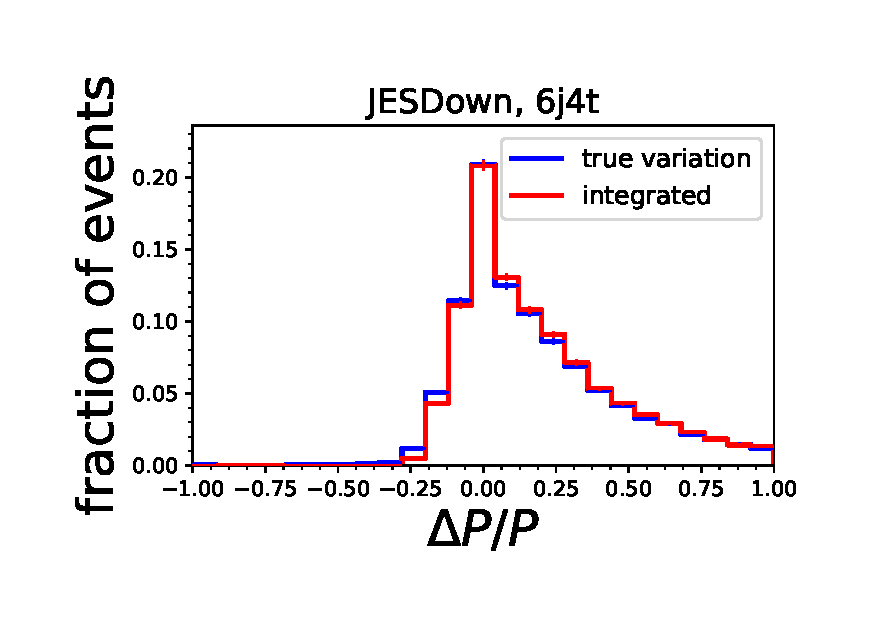
\includegraphics[width = 0.5\textwidth]{figures/mem/jesdown_variation.pdf}}\\
\caption[The distributions of the MEM signal and background probabilities]{The effect of JES variations up and down variations on the MEM signal probability for the signal hypothesis with the full computation (blue) and with the vector integration approximation method. We see that both the up and down shifts have the correct direction and magnitude. This estimation is done on~\ttHbb~simulation with exactly 6 jets and exactly 4 b~tags, requiring that the jet variations do not change the jet multiplicity in the final state.}
\label{fig:jes_variation}
\end{centering}
\end{figure}

Additional complexity is introduced due to variations in the uncertainties possibly changing the topology of the reconstructed final state, as scaling jet energies down may cause jets to migrate under the experimental threshold~$p_{T\mathrm{cut}}$. In order to account for this, in case a particular variation~$\vec{y} + \delta \vec{y}_n$ changes the reconstructed final state, the MEM is still recomputed using the new topology. On~\cref{fig:jes_variation_ratio}, we compare the fully variated MEM discriminator to the approximation, taking into account these jet multiplicity migrations.

\begin{figure}[ht]
\begin{centering}
\subfloat[Up-variation]{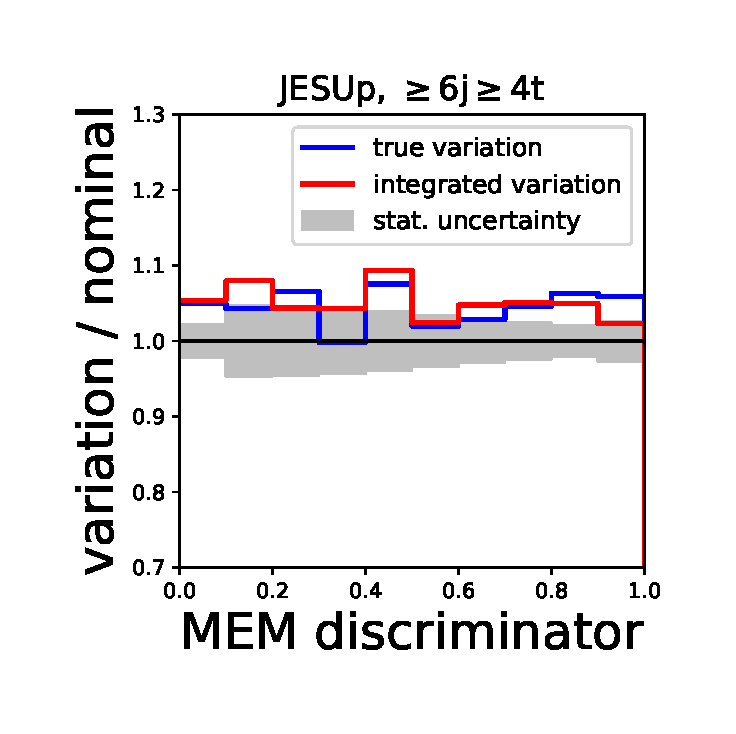
\includegraphics[width = 0.5\textwidth]{figures/mem/jesup_ratio_mem.pdf}}
\subfloat[Down-variation]{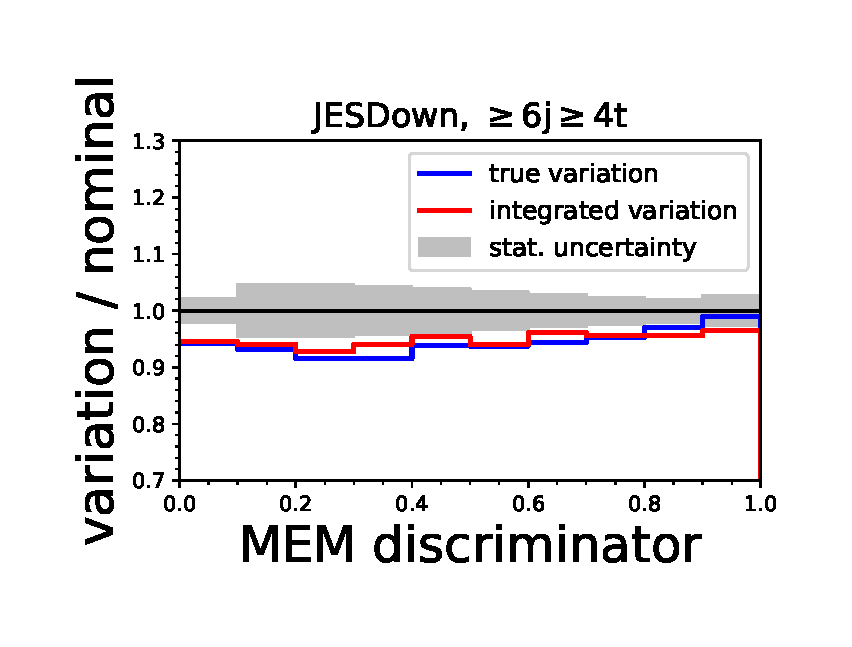
\includegraphics[width = 0.5\textwidth]{figures/mem/jesdown_ratio_mem.pdf}}\\
\caption[The full variation in the MEM discriminator]{The effect of JES variations up and down variations on the MEM discriminator (likelihood ratio) with the full computation (blue) and with the vector integration approximation method. As before, We see that both the up and down shifts have the correct direction and magnitude. The differences are not significant, compared to the MC statistical uncertainty. This estimation is done on~\ttHbb~simulation with at least 6 jets and at least 4 b~tags, taking into account possible bin-to-bin migrations.}
\label{fig:jes_variation_ratio}
\end{centering}
\end{figure}

\subsection{MEM on the WLCG}

From the computational cost of the MEM shown in~\cref{sec:mem_computational}~it is apparent that it is necessary to use distributed computing systems in order to have a reasonable turn-around time for the analysis. Therefore, we have parallelized the workflow both on the level of a computing cluster using \texttt{grid-control} and the WLCG using \texttt{CRAB}. On the WLCG, we have thus been able to take advantage of CMS computing resources opportunistically and have demonstrated that the MEM as implemented here is able to run on a wide range of data centres on a planetary scale. For this, we relied on \texttt{CMSSW} to provide a consistent environment along with user-provided external dependencies such as \texttt{OpenLOOPS}. We integrated the MEM into a multi-step workflow that produced the final analysis data sets directly from the CMS MiniAOD data stage in a single pass on the WLCG. This way, we were able to benefit from load balancing using data locality in CMS and reduced the number of manual intermediate steps and data management, which can be error prone. Overall, we were able to iterate with the full analysis from MiniAOD to the final limits in a matter of a few days.

\section{Expected performance}
\label{sec:mem_performace}
We study the expected performance of the MEM on a MC simulation sample of~\ttHbb~and \ttbar+jets. First, on~\cref{fig:mem_proba}, we verify that the signal and background probabilities indeed behave as expected on their respective MC simulations. In particular, we see that the signal probability is on average higher on the~\ttHbb~sample and vice versa, as we would expect. This allows us to construct an efficient likelihood ratio discriminator in the form

\begin{equation}
\lambda(\mathbf{y}) = \frac{P_{\mathrm{sig}}(\vec{y})}{P_{\mathrm{sig}}(\vec{y}) + \alpha \cdot P_{\mathrm{bkg}}(\vec{y})}
\end{equation}
The scale factor~$\alpha$~is optimised to adjust the relative normalization of the signal and background probabilities and is introduced to allow the dynamic range of~$P_{\mathrm{s}/\mathrm{b}}$~to be uniform in the range~$P_{\mathrm{s}/\mathrm{b}} \in [0, 1]$. Adjusting this coefficient does not change the signal-to-background discrimination power of the discriminant as it is a monotonic rescaling, but allows us to discretize the distribution into a small number of bins without losing sensitivity.

\begin{figure}[ht]
\begin{centering}
\subfloat[MEM probability for the~\ttH~hypothesis.]{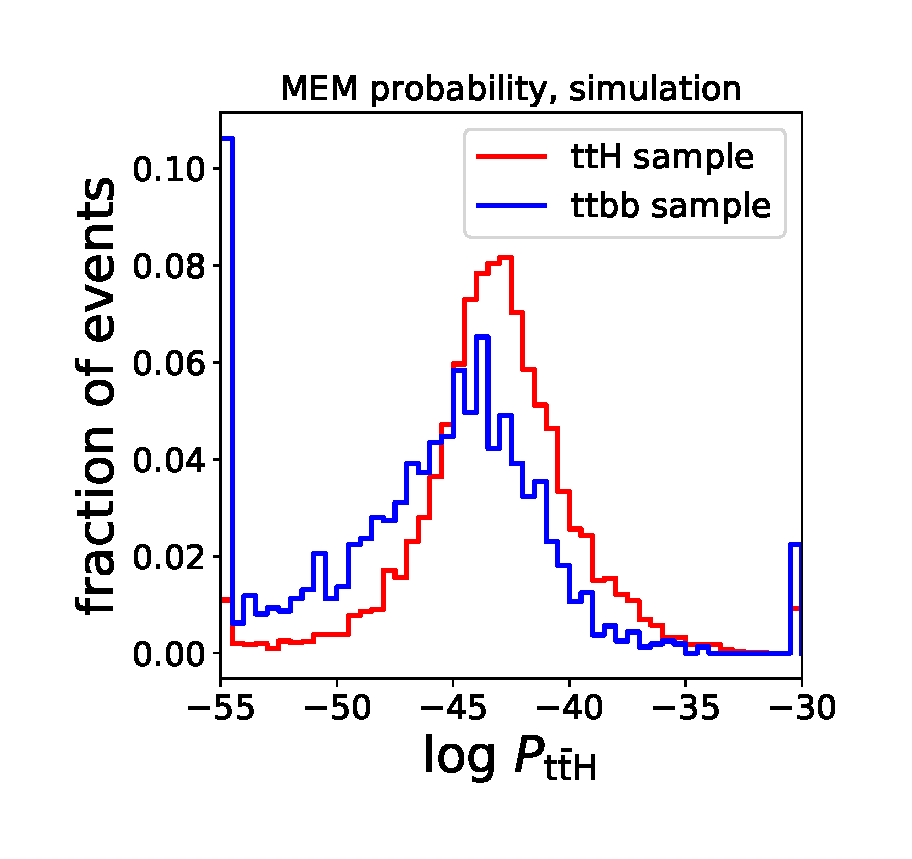
\includegraphics[width = 0.5\textwidth]{figures/mem/mem_proba_tth.pdf}}
\subfloat[MEM probability for the~\ttbb~hypothesis]{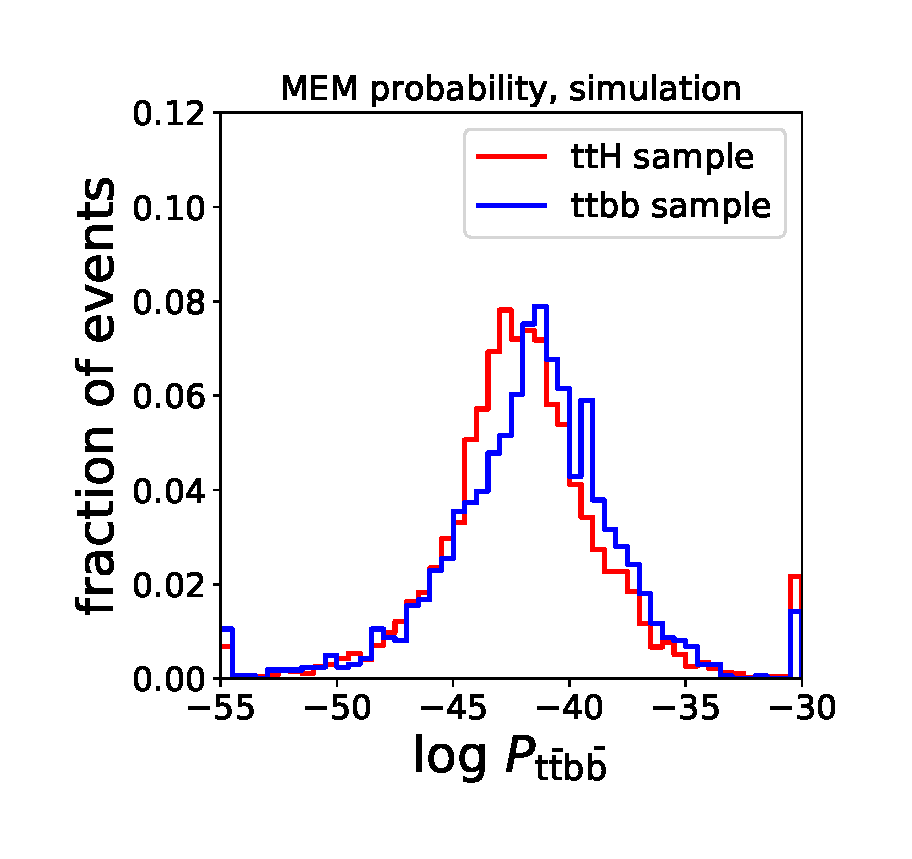
\includegraphics[width = 0.5\textwidth]{figures/mem/mem_proba_ttbb.pdf}}\\
\caption[The distributions of the MEM signal and background probabilities]{The expected distribution of the signal probability~$P_{\ttHbb}$ and the background probability~$P_{\ttbb}$ on MC simulation. We see that for the signal sample, the signal probability is on average higher than the background probability, and vice versa for the background. Here, we have selected events with exactly 1 isolated lepton, at least 6 jets, out of which 4 must be b~tagged. Furthermore, the jets are required to be matched to quarks from the corresponding hard interaction on generator level.}
\label{fig:mem_proba}
\end{centering}
\end{figure}

The performance of the MEM depends crucially on whether the jets in the observed final state can be correctly associated to the particles from the hard interaction. For the following comparisons, we define the full~\ttHbb~selection, corresponding to all the events that pass the detector-level selection criteria; and the matched selection, where the full selection is augmented by further requiring that all the jets in the event can be matched to the generator-level partons of the corresponding to the hypothesis. This matching is done geometrically using a cone size of~$\Delta R = 0.3$.

For example, for the signal hypothesis in the~$2_{\mathrm{W}} 2_{\mathrm{h}} 2_{\mathrm{t}}$ interpretation, we require that the two light jets can be matched to the quarks from the hadronic W~decay, two b~jets can be matched to bottom quarks from the Higgs and two b jets to bottom quarks from the top quark decay. This is done using generator-level information using the full decay chain. For the~$1_{\mathrm{W}} 2_{\mathrm{h}} 2_{\mathrm{t}}$ hypothesis, we require only one of the light jets to be matched to a quark from the W~boson, and for the~$0_{\mathrm{W}} 2_{\mathrm{h}} 2_{\mathrm{t}}$~hypothesis, the only the b jets are  required to be matched to b quarks. We show the estimated matching fractions in~\cref{tab:matching_fracs}. We find that in the semileptonic~$\geq6j\geq4t$~category, the jets can be fully matched to the quarks in approximately 20\% of the cases, whereas in the dileptonic~$\geq4j\geq4t$~category, the fraction is 59\%, allowing the MEM computation to be more effective.

\begin{table}[h!]
\begin{center}
\begin{tabular}{c|ccccc}
\hline
category & hypothesis & full final state & Higgs and top & Higgs only \\
\hline
SL $\geq$6j$\geq$4t & SL $2_{\mathrm{W}} 2_{\mathrm{h}} 2_{\mathrm{t}}$ & 0.20 & 0.51 & 0.69 \\
SL $\geq$6j3t & SL $2_{\mathrm{W}} 2_{\mathrm{h}} 2_{\mathrm{t}}$ & 0.09 & 0.24 & 0.52 \\
SL 5j$\geq$4t & SL $1_{\mathrm{W}} 2_{\mathrm{h}} 2_{\mathrm{t}}$ & 0.36 & 0.59 & 0.74 \\
SL 5j3t & SL $1_{\mathrm{W}} 2_{\mathrm{h}} 2_{\mathrm{t}}$  & 0.14 & 0.23 & 0.51 \\
SL 4j4t & SL $0_{\mathrm{W}} 2_{\mathrm{h}} 2_{\mathrm{t}}$ & 0.61 & 0.61 & 0.75 \\
SL 4j3t & SL $0_{\mathrm{W}} 2_{\mathrm{h}} 2_{\mathrm{t}}$  & 0.18 & 0.18 & 0.47 \\
\hline
DL $\geq$4j$\geq$4t & DL $2_{\mathrm{h}} 2_{\mathrm{t}}$ & 0.59 & 0.59 & 0.74 \\
DL $\geq$4j3t & DL $2_{\mathrm{h}} 2_{\mathrm{t}}$ & 0.30 & 0.30 & 0.55 \\
\hline
\hline
\end{tabular}
\caption[The fraction of matched events in the analysis categories]{The fraction of events where the jets could be matched to partons from the hard interaction under the full hypothesis consisting of all the quarks from the W-boson, top and Higgs decay; matching only the b~quarks from the Higgs and top decay and finally only the quarks from the Higgs decay. We see that for the SL~$\geq6j\geq4t$~category, 20\% of events could be matched to the full final state, whereas in the DL~$\geq4j\geq4t$~category, the equivalent fraction is 59\%. This stark differences arises due to the difficulty of reconstructing light quarks from the hadronic W-boson decay. Furthermore, we see that in the categories with 3 b~tags, the fraction of events with full matching is significantly lower, especially in terms of matching for the top quark decay products. The estimation is made using~\ttHbb~simulation.}
\end{center}
\label{tab:matching_fracs}
\end{table}

\subsection{Semileptonic categories}
We compare the MEM distributions and expected performance on events with 4 jets, 5 jets and~$\ge6$ jets in the single-lepton channel. Using these 3 broad categories, we can see the effect of adding additional information about jet kinematics to the MEM discriminator. We further split the events into two subcategories requiring at least 4 b~tagged jets, corresponding to a high-purity selection, and exactly 3 b~tagged jets and a high~$\mathcal{BLR}$ discriminator, corresponding to a lower-purity MEM control region. This allows us to evaluate the effect of incorrect hypotheses on the MEM performance, as the lower-purity category will have a large fraction of events which cannot be matched according to the above prescription. 

\subsubsection{4-jet final state}
On the SL categories with only 4 jets using only the kinematics of the b~jets, we are able to achieve a background efficiency of~$\simeq 30\%$ at a signal efficiency of~$50\%$ by selecting a sample where the 4 jets are likely to arise from bottom quarks using b tagging, as seen on~\cref{fig:mem_sl_j4_t4}. Extending the MEM to the 3 b tag, high~$\mathcal{BLR}$ shows the importance of having selected the right candidates for the b quarks, as can be seen on~\cref{fig:mem_sl_j4_t3}, where the lower matching fraction in signal results in a lower discriminator performance. Therefore, we conclude that it is feasible to use the newly-introduced $0_{\mathrm{W}} 2_{\mathrm{h}} 2_{\mathrm{t}}$-hypothesis in the 4-jet category, in case the 4 jets are likely to arise from the hadronization b quarks from the decay of the Higgs boson and the top quark.

\begin{figure}[ht]
\begin{centering}
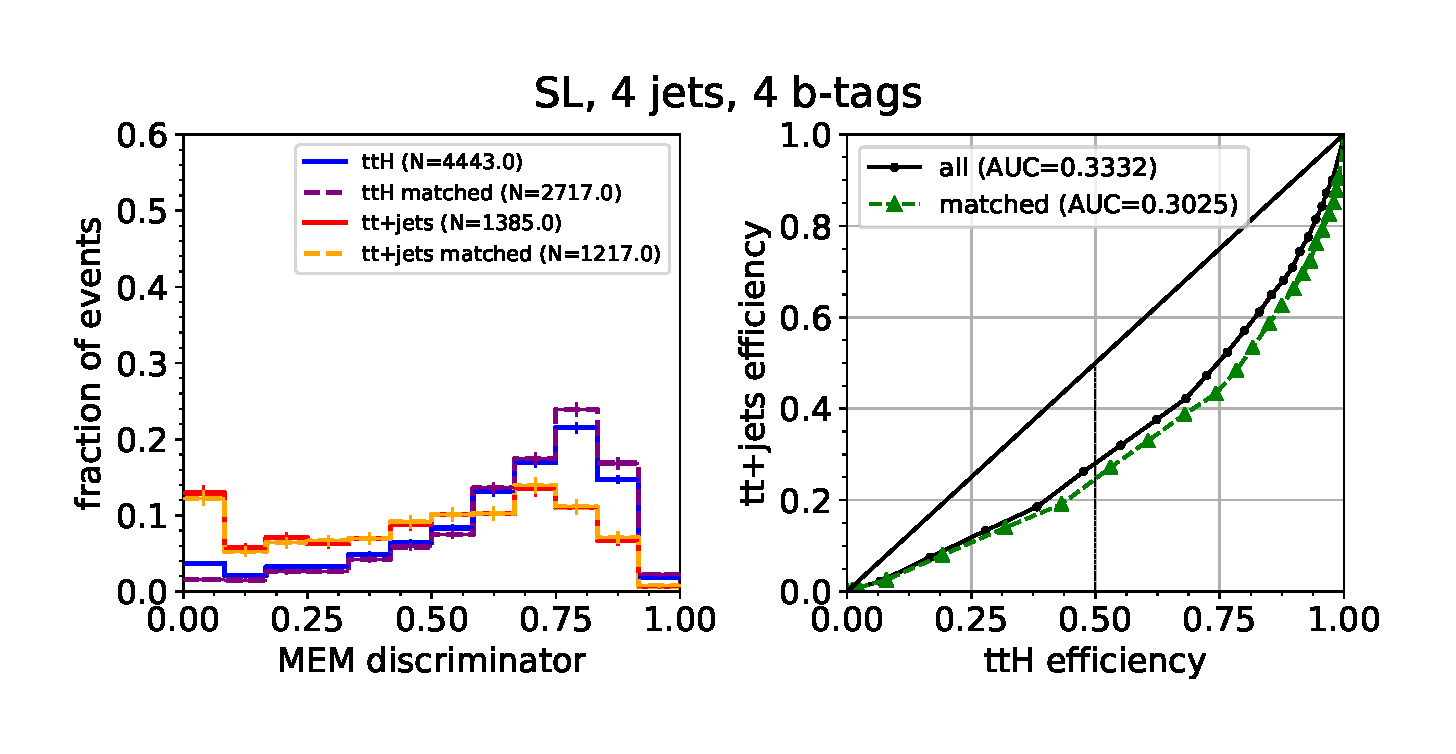
\includegraphics[width = 0.8\textwidth]{figures/mem/mem_sl_j4_t4.pdf}
\caption[MEM with the~$0_{\mathrm{W}} 2_{\mathrm{h}} 2_{\mathrm{t}}$ interpretation in the 4~jet, 4~b~tag category]{The MEM discriminator with the interpretation~$0_{\mathrm{W}} 2_{\mathrm{h}} 2_{\mathrm{t}}$, with the momenta of the 2 light quarks from the~$\mathrm{W}$-boson integrated over, in the single-leptonic category with 4 jets, 4 b tags. Compared to~\cref{fig:mem_sl_j4_t3}, we see an improvement in performance, as the requirement of 4 b tags enhances the fraction of events where the jets can be matched to quarks, thereby increasing the fraction of events where the correct MEM hypothesis is computed.}
\label{fig:mem_sl_j4_t4}
\end{centering}
\end{figure}

\begin{figure}[ht]
\begin{centering}
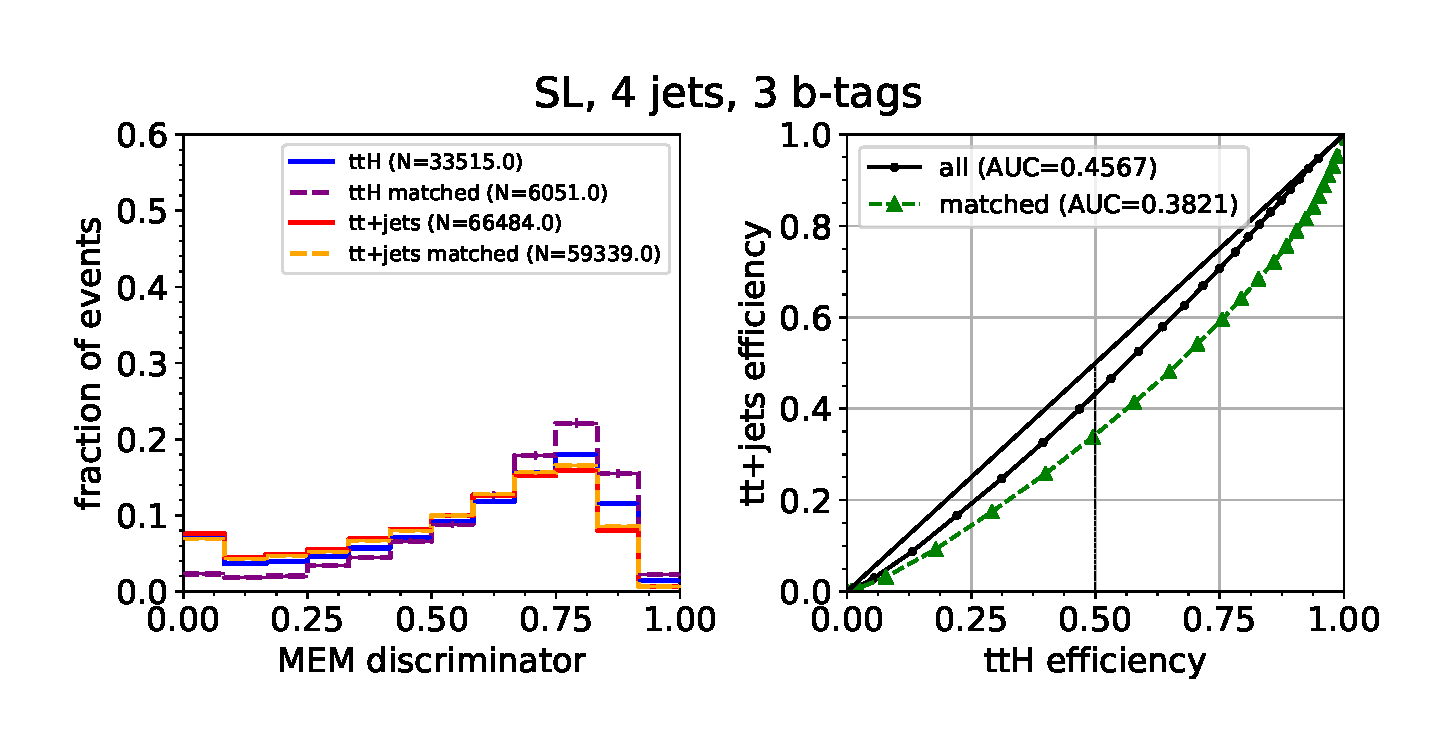
\includegraphics[width = 0.8\textwidth]{figures/mem/mem_sl_j4_t3.pdf}
\caption[MEM with the~$0_{\mathrm{W}} 2_{\mathrm{h}} 2_{\mathrm{t}}$ interpretation in the 4~jet, 3~b~tag category]{The MEM discriminator with the interpretation~$0_{\mathrm{W}} 2_{\mathrm{h}} 2_{\mathrm{t}}$, with the momenta of the 2 light quarks from the~$\mathrm{W}$-boson integrated over, in the single-leptonic category with 4 jets, 3 b tags. On the left, we show the discriminator distributions, on the right, the expected performance as characterized by the ROC for all events (black) and the events for which the jets could be matched to the partons from the hard process (green). Based on the kinematics of the 4 b jet, the MEM is already able to achieve a degree of separation ($\mathrm{AUC} = 0.41$) in this category. The distributions are derived using the full~\ttHbb~and~\ttbar+jets simulations, including detector effects.}
\label{fig:mem_sl_j4_t3}
\end{centering}
\end{figure}

\subsubsection{5-jet final state}
By adding the information of an additional jet in the 5 jet categories, the background efficiency decreases to~$20\%$ at the benchmark point of 50\% signal efficiency in the 4 tag category on~\cref{fig:mem_sl_j5_t4}. Thus we see that the additional information provided by the kinematics of the extra jet helps to constrain the MEM integration significantly. The category with 3 b tags and high~$\mathcal{BLR}$ performs slightly worse, with the main effect coming from the additional light jet not being associated to the~$\mathrm{W}$-boson, as can be seen from~\cref{fig:mem_sl_j5_t3}.

\begin{figure}[ht]
\begin{centering}
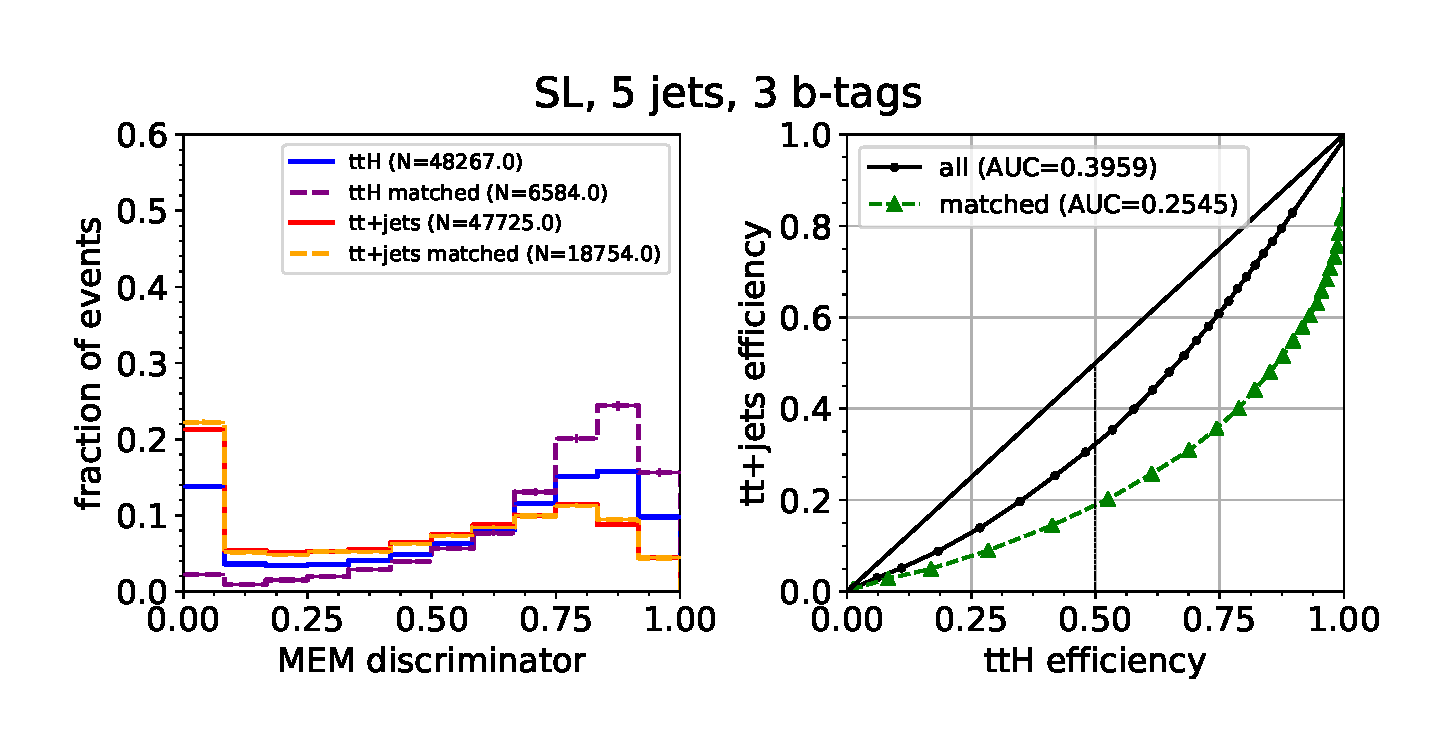
\includegraphics[width = 0.8\textwidth]{figures/mem/mem_sl_j5_t3.pdf}
\caption[MEM with the~$1_{\mathrm{W}} 2_{\mathrm{h}} 2_{\mathrm{t}}$ interpretation in the 5 jet, 3 b~tag category]{The MEM discriminator with the interpretation~$1_{\mathrm{W}} 2_{\mathrm{h}} 2_{\mathrm{t}}$, with the momentum of 1 of the light quarks from the~$\mathrm{W}$-boson integrated over, in the single-leptonic category with 5 jets, 3 b tags. Compared to~\cref{fig:mem_sl_j4_t3}, we have added the information about one of the quarks from the hadronic~$\mathrm{W}$-boson decay, thus constraining the integration. From the ROC on the right plot, we see that for the matched case (green), the MEM performs significantly better than the corresponding discriminator on~\cref{fig:mem_sl_j4_t3}, thanks to the additional information available. However, the low fraction of matched events ($< 10\%$ for signal) significantly degrades the observed performance (black). Most of the mismatched events come from the additional light quark not corresponding to the hadronic~$\mathrm{W}$-boson decay. Thus, we see the importance of deploying the MEM on final states where the relevant particles are reconstructed.}
\label{fig:mem_sl_j5_t3}
\end{centering}
\end{figure}

\begin{figure}[ht]
\begin{centering}
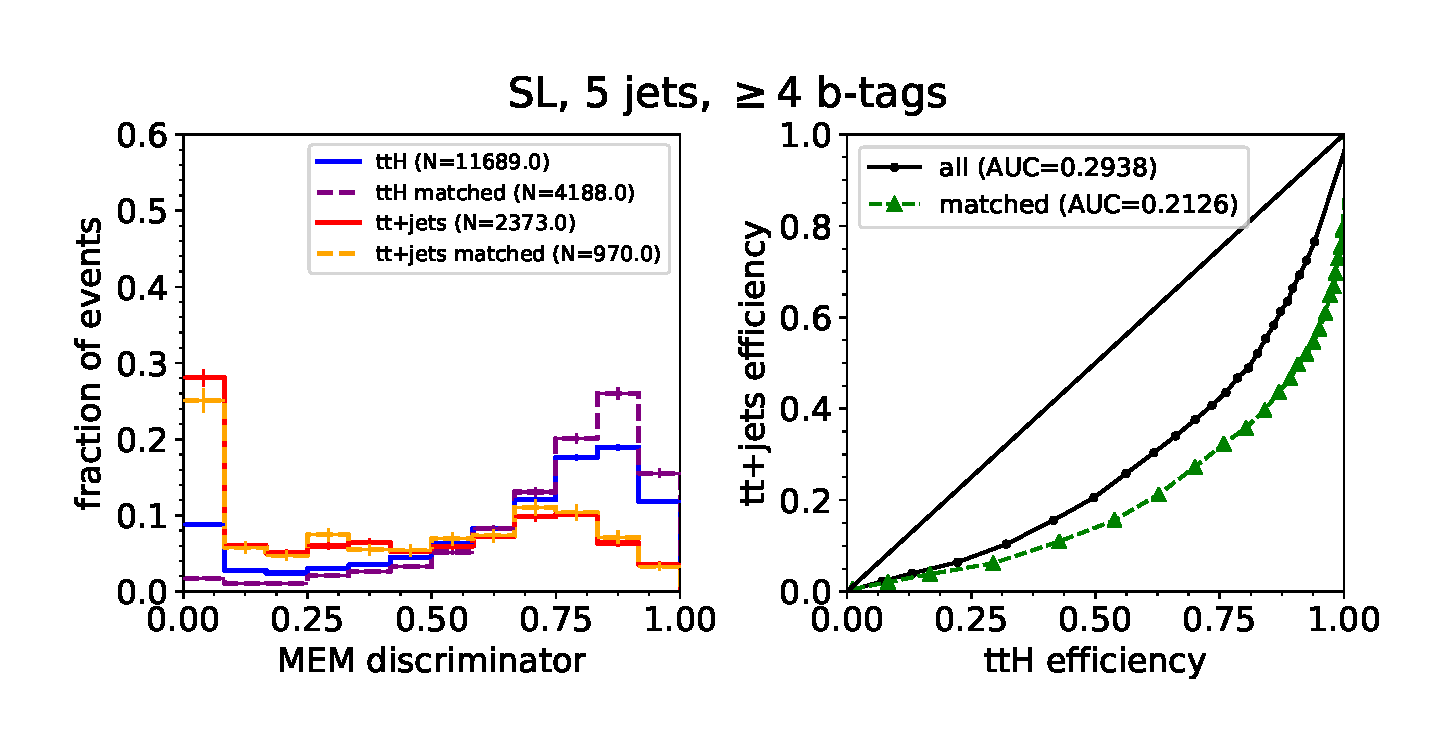
\includegraphics[width = 0.8\textwidth]{figures/mem/mem_sl_j5_tge4.pdf}
\caption[MEM with the~$1_{\mathrm{W}} 2_{\mathrm{h}} 2_{\mathrm{t}}$ interpretation in the 5 jet, $\ge4$ b~tags category]{The MEM discriminator with the interpretation~$1_{\mathrm{W}} 2_{\mathrm{h}} 2_{\mathrm{t}}$, with the momentum of 1 of the light quarks from the~$\mathrm{W}$-boson integrated over, in the single-leptonic category with 5 jets, 4 b tags. By requiring 4 b~tagged jets, the jets in the final state correspond to the partons from the underlying hypothesis in about~$35\%$ of cases for signal. We also see that the performance of the MEM discriminator is thus increased compared to~\cref{fig:mem_sl_j5_t3}.}
\label{fig:mem_sl_j5_t4}
\end{centering}
\end{figure}

\subsubsection{6-jet final state}
In the categories with 6 or more jets, we verify that the MEM is able to exploit the information in the fully-reconstructed category, with a~$\simeq 10\%$ background efficiency in the case where the jets could be fully matched to the partons of the underlying hypothesis, as shown on~\cref{fig:mem_sl_jge6_tge4} for events with at least 4 b~tagged jets. On the extended events with 3 b~tagged jets, high~$\mathcal{BLR}$, the MEM still shows relatively good discrimination (\cref{fig:mem_sl_jge6_t3}), with the most significant reduction coming from the fraction of events where one of the light jets assumed to arise from~$\mathrm{W} \rightarrow \mathrm{q} \mathrm{q}'$ was instead spurious.

\begin{figure}[ht]
\begin{centering}
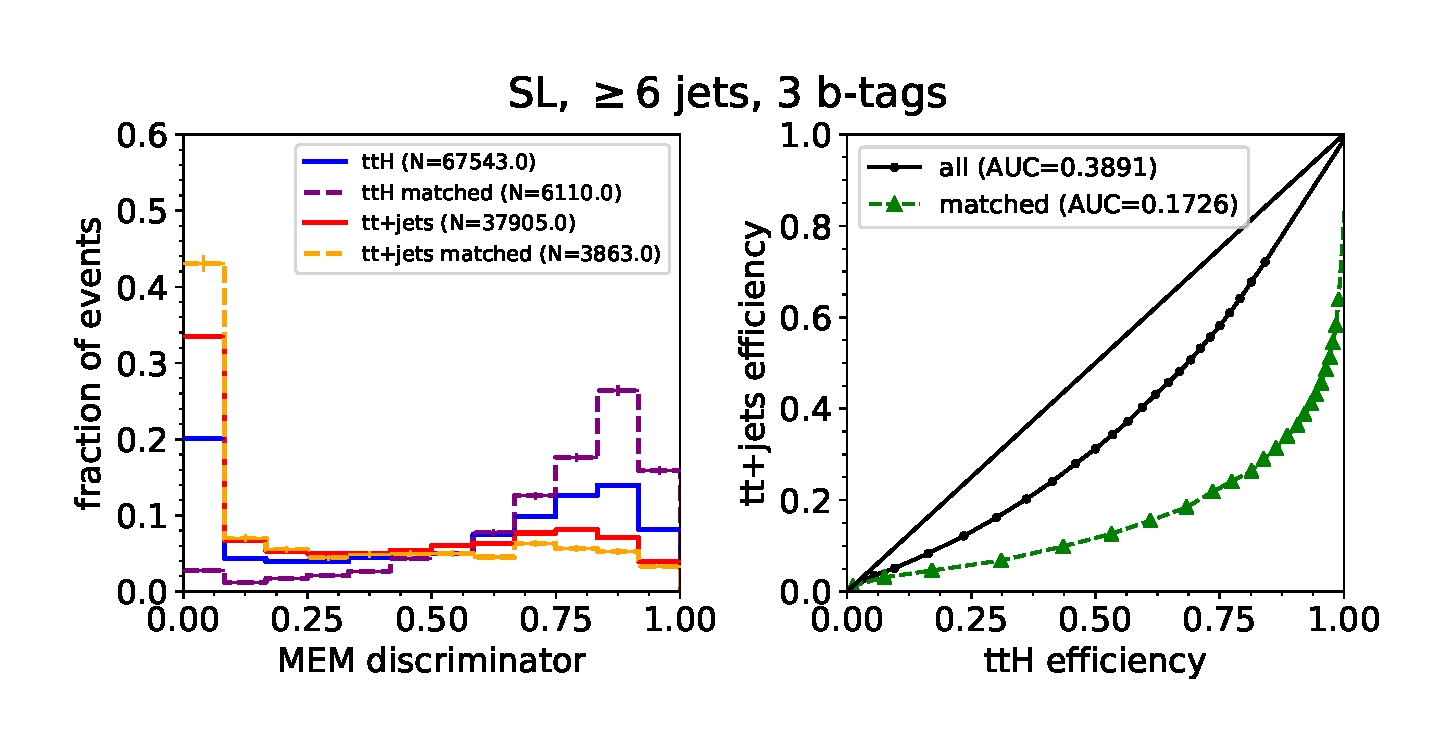
\includegraphics[width = 0.8\textwidth]{figures/mem/mem_sl_jge6_t3.pdf}
\caption[MEM with the $2_{\mathrm{W}} 2_{\mathrm{h}} 2_{\mathrm{t}}$ interpretation in the $\ge6$ jets, 3~b tags category]{The MEM discriminator with the interpretation~$2_{\mathrm{W}} 2_{\mathrm{h}} 2_{\mathrm{t}}$, i.e. the fully reconstructed hypothesis, in the single-leptonic category with at least 6 jets, 3 b tags. We see that while the performance on the events that can be matched to the quarks from the underlying hard process is excellent, the fraction of matched events is below 10\%, degrading the performance on realistic events.}
\label{fig:mem_sl_jge6_t3}
\end{centering}
\end{figure}

\begin{figure}[ht]
\begin{centering}
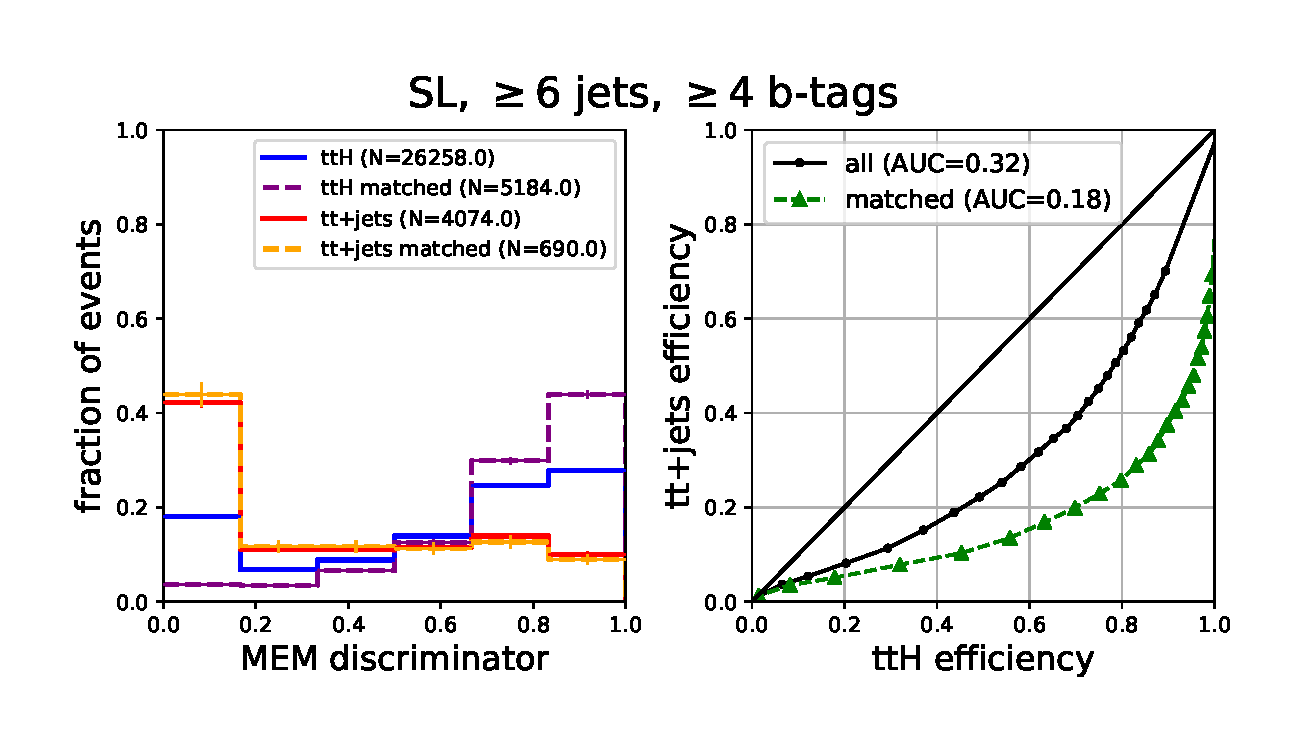
\includegraphics[width = 0.8\textwidth]{figures/mem/mem_sl_jge6_tge4.pdf}
\caption[MEM with the~$2_{\mathrm{W}} 2_{\mathrm{h}} 2_{\mathrm{t}}$ interpretation in the $\ge6$ jet, $\ge4$ b~tag category]{The MEM discriminator with the interpretation~$2_{\mathrm{W}} 2_{\mathrm{h}} 2_{\mathrm{t}}$, i.e. the fully reconstructed hypothesis, in the single-leptonic category with at least 6 jets, at least 4 of which must be b~tagged. This is the category with the highest signal to background ratio and with a full reconstruction of the 2 light quark, 4 bottom quark final state corresponding to~\ttHbb. We see that in case all the jets were matched to the quarks, the signal to background separation provided by the MEM is significant, with a background efficiency of around~$10\%$ at a median signal efficiency. After relaxing the matching criterion, the separation decreases by about a factor of 2 at the expense of the signal distribution becoming more background-like.}
\label{fig:mem_sl_jge6_tge4}
\end{centering}
\end{figure}

\subsubsection{Mis-reconstructed events in the 6-jet categories}
Motivated by the significant effect on the MEM from the unmatched jets, we investigate a possibility to mitigate the effect within the discriminator by integrating over the jet momenta in case we are unsure if they correspond to the object on the level of the hard scattering. In particular, since we have seen that a significant fraction of the light jets in the fully-reconstructed category are not matched to the quarks from the W-boson decay, we consider relaxing the assumption that all the light quarks are reconstructed as jets.

This amounts to applying an interpretation such as~$1_{\mathrm{W}} 2_{\mathrm{h}} 2_{\mathrm{t}}$ that only uses the kinematics of 5 jets on an event with 6 or more jets. In general, we see that for realistic detector-level events without generator-level matching, this strategy results in a slightly improved performance, due to being less sensitive to the mis-reconstruction of the light jets, as can be seen comparing~\cref{fig:mem_sl_jge6_tge4_1w2h2t} and~\cref{fig:mem_sl_jge6_tge4}. In particular, the ROC AUC performance characteristic for the unmatched events decreases from $\mathrm{AUC} = 0.32$ to $\mathrm{AUC} = 0.31$ and the difference between the~\ttHbb~MEM distribution between the matched and unmatched event samples decreases.

However, the computational cost~(\cref{tab:mem_cpu_budget})~would increase by about a factor of 2 with this choice, therefore, we do not use this approach in the~\ttHbb~analysis at this stage. In the future, it may be interesting to explore complex hypothesis tests, which effectively combine the probabilities under various jet reconstruction hypotheses in a uniform way, smoothly interpolating between a fully-reconstructed and a partially reconstructed hypothesis based on some event-level observables.

\begin{figure}[ht]
\begin{centering}
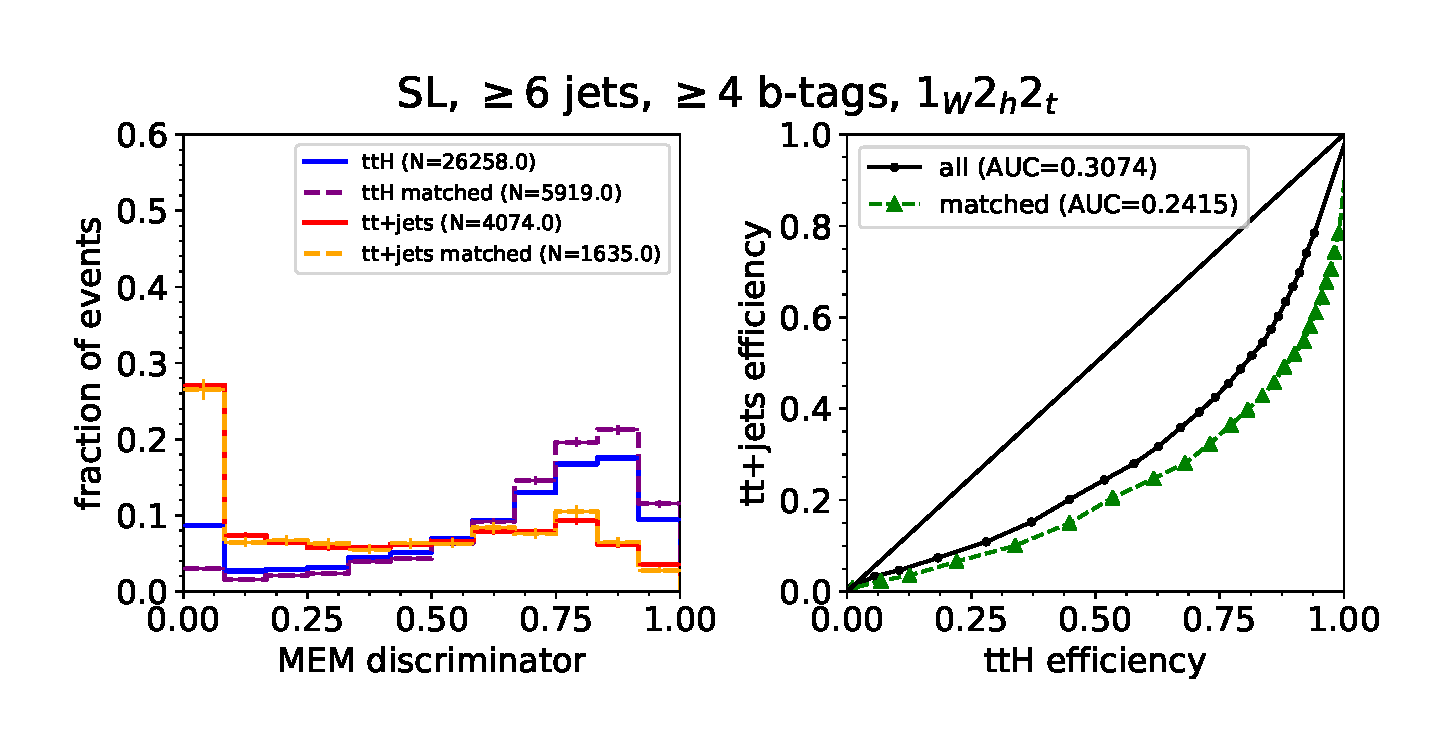
\includegraphics[width = 0.8\textwidth]{figures/mem/mem_sl_jge6_tge4_1w2h2t.pdf}
\caption[MEM with the~$1_{\mathrm{W}} 2_{\mathrm{h}} 2_{\mathrm{t}}$ interpretation in the $\ge6$ jet, $\ge4$ b~tag category]{The MEM discriminator with the interpretation~$1_{\mathrm{W}} 2_{\mathrm{h}} 2_{\mathrm{t}}$ in the single-leptonic category with at least 6 jets, at least 4 of which must be b~tagged. In comparison to~\cref{fig:mem_sl_jge6_tge4}~, we have integrated over the momentum of one of the light jets, assuming that only one of the two light jets corresponds to a quark from the~$\mathrm{W}$-boson decay. We see a slightly improved performance compared to the fully reconstructed hypothesis in the case of all events (black), and a slight decrease for events that are fully matched. This is consistent with the performance of the MEM being strongly dependent on whether the objects in the final state correspond to the hard scattering process.}
\label{fig:mem_sl_jge6_tge4_1w2h2t}
\end{centering}
\end{figure}

\subsubsection{7-jet categories}
Furthermore, we have studied the effect of including diagrams containing additional radiation, as outlined in~\cref{sec:mem_radiation}. These additional diagrams are only valid on events with at least 7 jets. We have compared the standard fully reconstructed hypothesis on~\cref{fig:mem_sl_jge7_tge4} to the one with additional gluon radiation on~\cref{fig:mem_sl_jge7_tge4_7jet} in this category. We see that using the diagram for additional radiation has a very small effect on the final discrimination, since the effect of spurious jets incorrectly assigned to the hadronic W-boson decay is significantly larger than that of the better description provided by the accurate treatment of the additional radiation. From this, we conclude that the most straightforward way to improve the performance of the MEM discriminator is to ensure that the hypothesis corresponds to the particles reconstructed in the final state. Therefore, we consider this as a cross-check of the MEM and do not investigate it further in the~\ttHbb analysis.

\begin{figure}[ht]
\begin{centering}
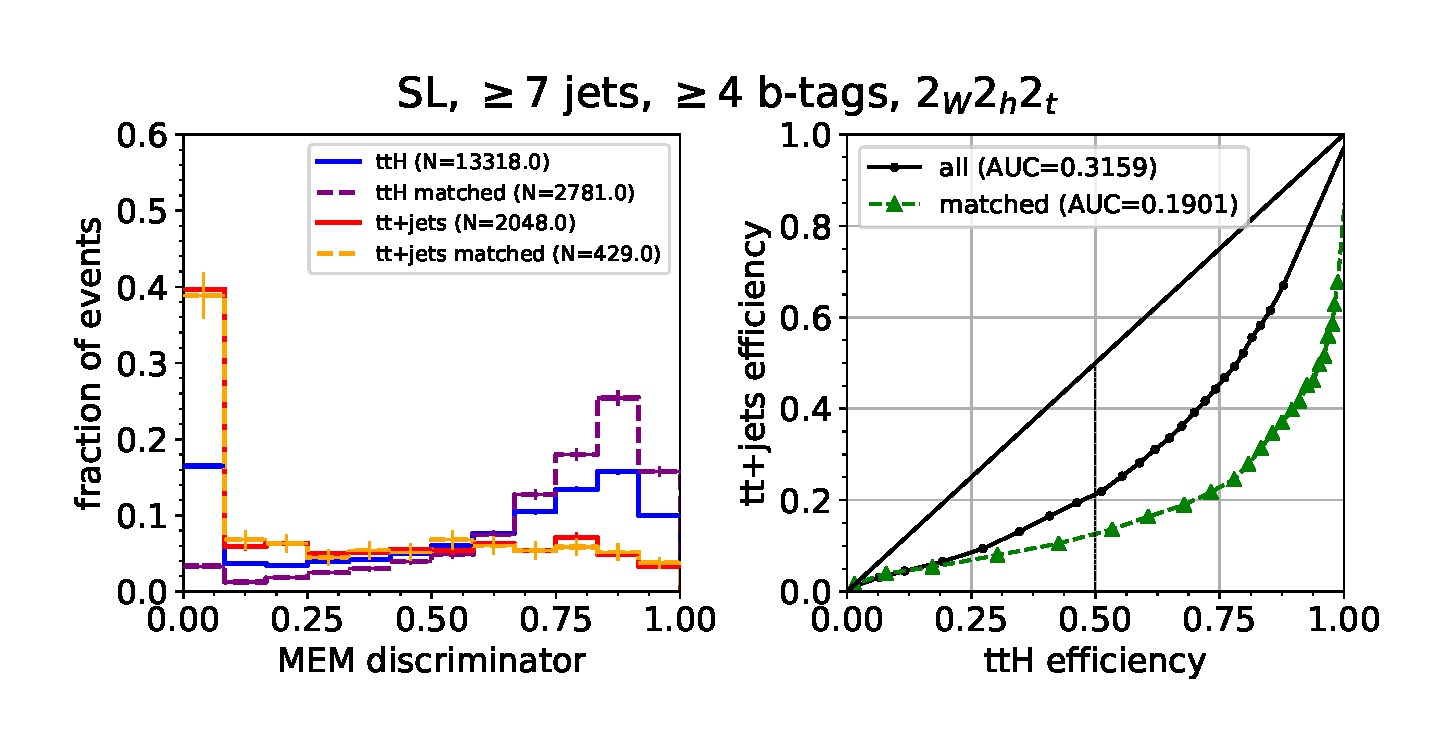
\includegraphics[width = 0.8\textwidth]{figures/mem/mem_sl_jge7_tge4.pdf}
\caption[MEM with the~$2_{\mathrm{W}} 2_{\mathrm{h}} 2_{\mathrm{t}}$ interpretation in the $\ge7$-jet, $\ge4$ b~tag category]{The MEM discriminator with the interpretation~$2_{\mathrm{W}} 2_{\mathrm{h}} 2_{\mathrm{t}}$, i.e. the fully reconstructed interpretation, in the single-leptonic category with at least 7 jets, at least 4 of which must be b~tagged. In order to interpret the light jets as quarks, we sum over all possibilities of choosing 2 light quarks from the 3 light jets most compatible with a~$\mathrm{W}$-boson decay according to invariant mass. We see that in the presence of an additional jet, the fully-reconstructed MEM interpretation is still able to distinguish between signal and background at an acceptable level.}
\label{fig:mem_sl_jge7_tge4}
\end{centering}
\end{figure}

\begin{figure}[ht]
\begin{centering}
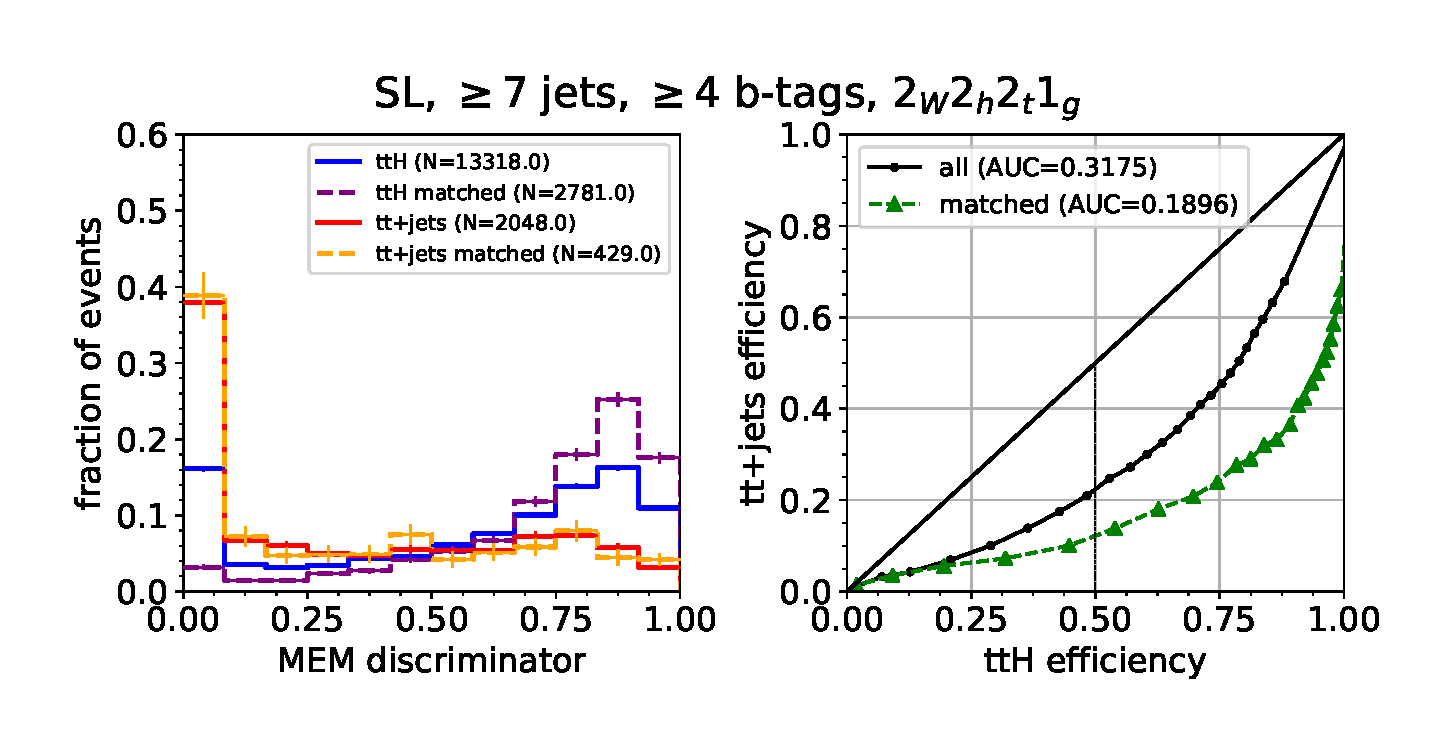
\includegraphics[width = 0.8\textwidth]{figures/mem/mem_sl_jge7_tge4_1g.pdf}
\caption[MEM with the~$2_{\mathrm{W}} 2_{\mathrm{h}} 2_{\mathrm{t}} 1_{\mathrm{g}}$ interpretation in the $\ge7$ jet, $\ge4$ b~tag category]{The MEM discriminator with the interpretation~$2_{\mathrm{W}} 2_{\mathrm{h}} 2_{\mathrm{t}} 1_{\mathrm{g}}$, where we include the gluon radiation in the signal and background hypotheses, in the single-leptonic category with at least 7 jets, at least 4 of which must be b~tagged. Compared to the hypothesis without gluon radiation on~\cref{fig:mem_sl_jge7_tge4}~, we do not see an improved discrimination from including this more complex hypothesis.}
\label{fig:mem_sl_jge7_tge4_7jet}
\end{centering}
\end{figure}

\subsection{Dileptonic categories}
We have also evaluated the MEM discriminator in the dileptonic categories, where the W-bosons from both top quarks decay leptonically. At the level of the hard interaction, we expect 4 b~quarks: two from the \Hbb~decay and 2 from the top quark decay. In order to associate the jets to the quarks, we select the set of 4 jets that are most compatible with b~quarks. Thus, we have 12 combinations to assign the 4 quarks to the 4 b jets. In general, we see excellent performance of the MEM in the dilepton categories with both 4 and 3 b~tags, since in around 60\% of the cases, the jets in the event can be matched to the b~quarks from the underlying hard process. This means that the MEM can be used as a powerful signal-to-background discriminator in the dilepton final states, despite the complexity of the integration that is required to account for the momenta of the two neutrinos.


\begin{figure}[ht]
\begin{centering}
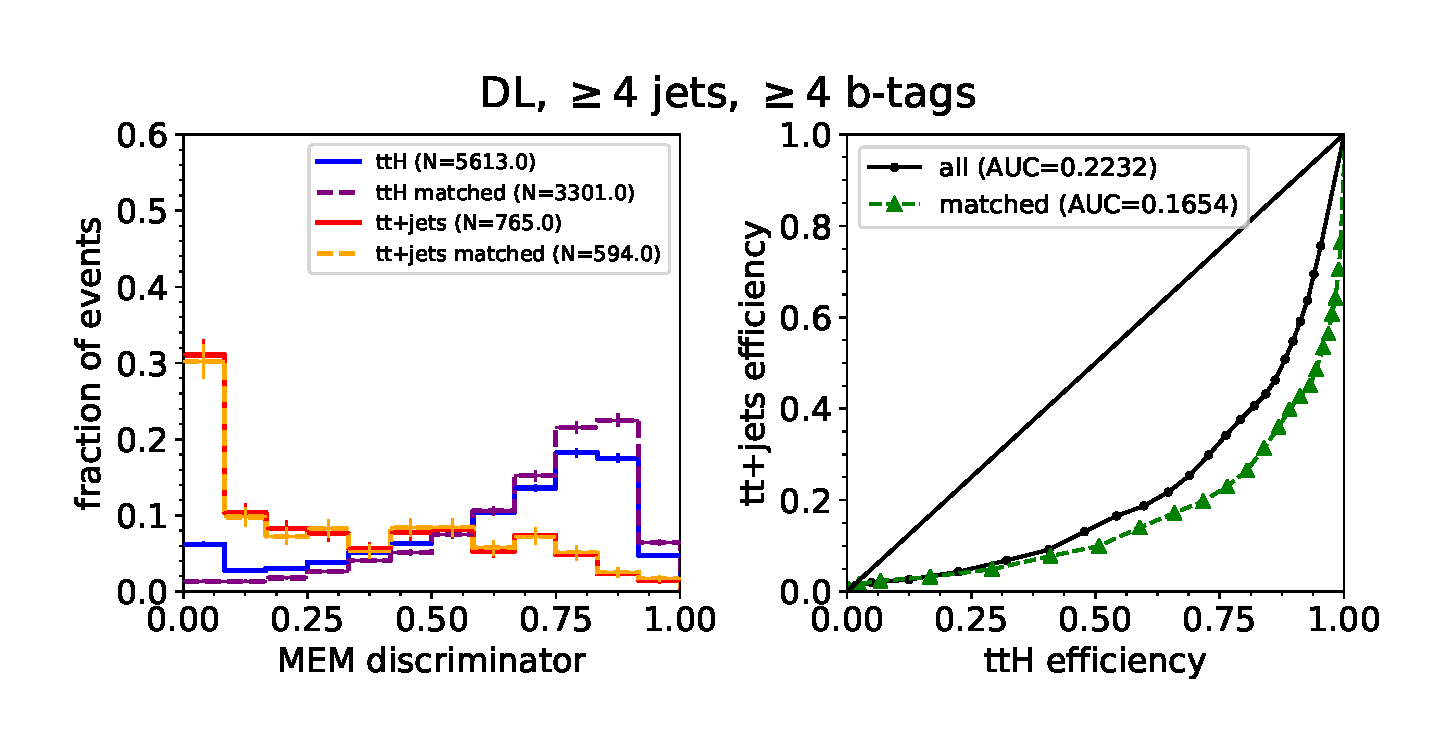
\includegraphics[width = 0.8\textwidth]{figures/mem/mem_dl_jge4_tge4.pdf}
\caption[MEM with the~$2_{\mathrm{h}} 2_{\mathrm{t}}$ interpretation in the dileptonic $\ge4$ jet, $\ge4$ b~tag category]{The MEM discriminator with the interpretation~$2_{\mathrm{h}} 2_{\mathrm{t}}$ in the dileptonic category with at least 4 jets, all of which must be b~tagged. We see that at 50\% signal efficiency, the inclusive~\ttbar~efficiency is around 17\% as estimated on simulation.}
\label{fig:mem_dl_jge4_tge4}
\end{centering}
\end{figure}

\begin{figure}[ht]
\begin{centering}
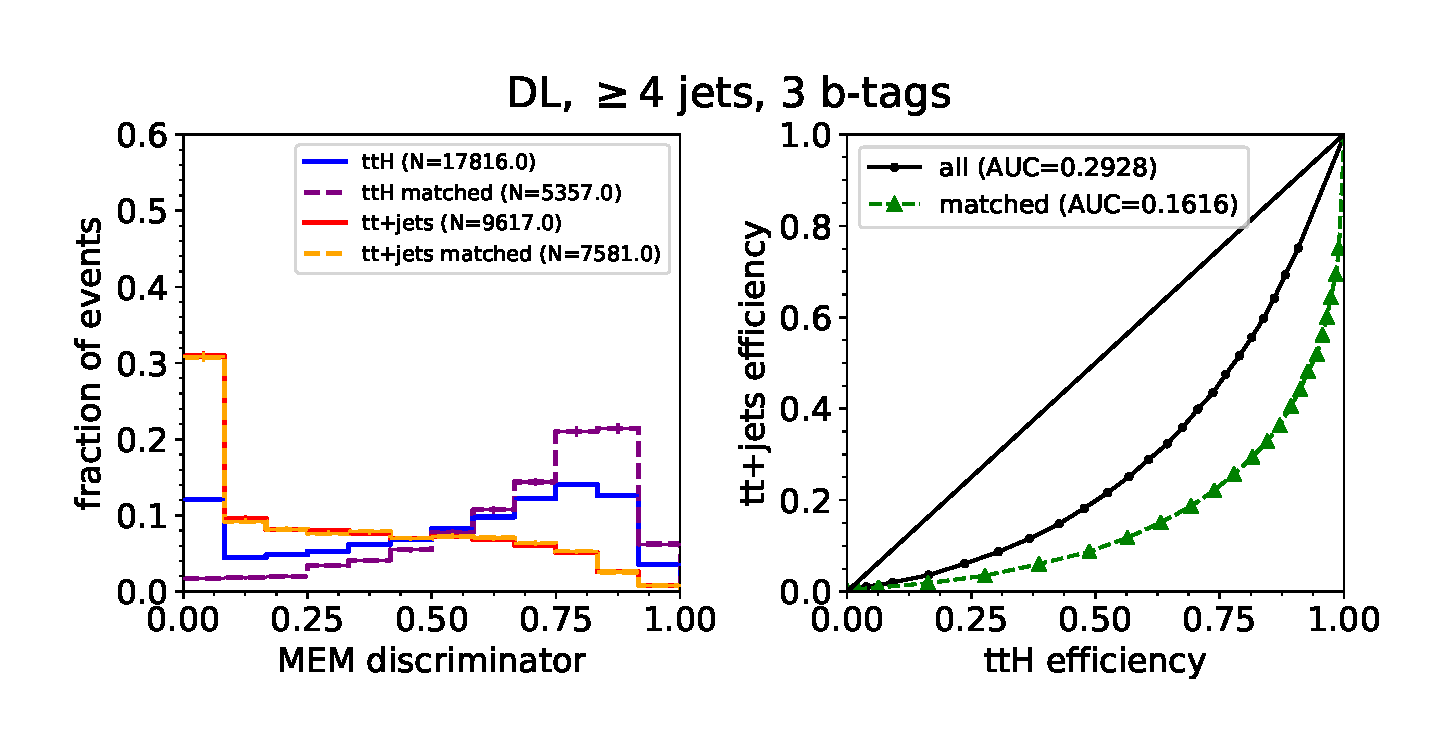
\includegraphics[width = 0.8\textwidth]{figures/mem/mem_dl_jge4_t3.pdf}
\caption[MEM with the~$2_{\mathrm{h}} 2_{\mathrm{t}}$ interpretation in the dileptonic $\ge4$ jet, 3 b~tag category]{The MEM discriminator with the interpretation~$2_{\mathrm{h}} 2_{\mathrm{t}}$ in the dileptonic category with at least 4 jets, out of which 3 are b~tagged. Compared to~\cref{fig:mem_dl_jge4_tge4}, the expected performance decreases somewhat, with a background efficiency of 20\% at the reference signal efficiency. Nevertheless, it is possible to use the DL MEM in the 3 b~tag category as an efficient tt+bb discriminator.}
\label{fig:mem_dl_jge4_t3}
\end{centering}
\end{figure}

\section{Summary of MEM studies}
To summarize, we have implemented the MEM discriminator for the~\ttHbb~analysis in Run II with significant improvements over the approach used in Run I. The MEM can now be computed in all relevant final states in the~\ttHbb~analysis and we have studied the expected performance on MC simulation. The performance studies are carried out in several categories with a varying number of jets, corresponding to the gradual increase of information available to the MEM in a multi-particle final state. We have seen that in case all the partons from the hard scattering process are present in the final state, the MEM is able to distinguish between the signal and background hypotheses with a background efficiency of~$\simeq 10\%$ for a signal efficiency of~$50\%$ based only on high-level event kinematic properties. The effect of the quark jets being outside the acceptance region degrades the performance of the discriminator, as the spurious jets that are instead associated to the quarks do not provide any constraining power in the integrand. Therefore, an accurate reconstruction of the final state is very important for the MEM discriminator, especially in the signal sample.

Nevertheless, the expected realistic performance of the MEM, based on full detector simulation, is excellent in the high jet and b~tag multiplicity categories. In the best semileptonic category, the \ttbar+jets efficiency is around 20\% at a reference signal efficiency of 50\%, whereas in dilepton, the background rejection is even higher. We have further studied the resilience of the MEM to QCD radiation and found that the performance does not change markedly by introducing effective Sudakov reweighting or diagrams with additional jets. In conclusion, we find that the MEM is a suitable discriminator in the~\ttHbb~search, given the performance and the solid theoretical foundation on which it is based.
